\section[The noncoding genome]{The noncoding genome}
\label{sec:noncoding-genome}

One of the distinguishing hallmarks of eukaryotic genomes is their large size and low protein-coding content. Less than 2\% of the human genome consists of protein-coding genes.\autocite{djebali_2012_landscape} The question then arises as to the composition and function (if any) of the remaining genome.

Much of the noncoding regions of the human genome have historically been called "\textit{junk DNA}". Transcriptome genome-wide analyses over the past 18 years demonstrated that regions between protein-coding genes are frequently transcribed into RNA molecules of diverse lengths.\autocite{kapranov_2007_lncRNA,guttman_2009_chromatin,derrien_2012_gencode,brown_2014} The various types of non-protein-coding loci can be classified according to its length into: \textbf{1)} short (< 200 nucleotides) and \textbf{2)} long noncoding RNAs (> 200 nucleotides).

\begin{enumerate}
\item \textbf{Short noncoding RNAs}: carry out relative well-defined functions in cells, and are already accepted as fundamental players in gene regulation;\autocite{ulitsky_2018_interactions,pelechano_2013} these include: microRNAs (miRNAs), small nucleolar RNAs (snoRNAs), Piwi-interacting RNAs (piRNAs), small nuclear RNAs (snRNAs), tRNAs, and rRNAs. Conversely, short noncoding RNAs represent a tiny fraction of the human, mouse, and fruit fly genomes (see \autoref{tab:ncRNAs}). Usually short noncoding RNAs are recognized by 3D conformations by various proteins forming ribonucleoprotein complexes.\autocite{jarroux_2017_history,ulitsky_2018_interactions} 

\item \textbf{Long noncoding RNAs}: are the most common class of noncoding RNAs. Long noncoding RNAs (lncRNAs) are defined as RNAs longer than 200 nucleotides with no apparent coding potential. This poor definition encompasses a large and heterogeneous class of transcripts that differ in their biogenesis and genomic location, this poor definition comes from our limited understanding of lncRNAs. The majority of lncRNAs are transcribed by RNA polymerase II (Pol II) and often capped by 7-methyl guanosine (m$^7$G) at their 5’ ends, polyadenylated at their 3’ ends, and spliced similarly to protein-coding genes (PCGs).\autocite{statello_2021_lncRNA_reg,kopp_2018_functional} It is worthwhile highlighting that enhancer regions are also transcribed into enhancer RNAs (eRNAs).\autocite{statello_2021_lncRNA_reg,kim_2015_erna}

\end{enumerate}

\begin{table}[!htb]
  \caption[Short noncoding RNAs in the human, mouse and fruit fly genomes]{\textbf{Short noncoding RNAs in the human, mouse and fruit fly genomes}. Statistics are based on the following short noncoding RNAs: miRNAs, rRNAs, snoRNAs, snRNAs, and tRNAs.}
  \begin{scriptsize}
    \begin{tabulary}{0.65\linewidth}{ccccc}
      \textbf{Organism} & \textbf{Gene number} & \textbf{Genomic coverage (Kb)} & \textbf{Genome sequence covered} & \textbf{Annotation} \\ \hline
      Human & 8,130 & 783 & 0.027\% & GENCODE\autocite{frankish_2021_gencode} \\
      Mouse & 6,656 & 568 & 0.031\% & GENCODE\autocite{frankish_2021_gencode} \\
      Fruit fly & 1,019 & 161 & 0.134\% & FlyBase\autocite{thurmond_2019_flybase} \\
    \end{tabulary}
  \end{scriptsize}
  \label{tab:ncRNAs}
\end{table}

LncRNAs in contrast with short noncoding RNAs, are highly abundant and except for a few lncRNAs their function remains elusive; even with the constant efforts by reference annotations of coding and noncoding genes, including GENCODE\autocite{frankish_2021_gencode} or FlyBase\autocite{thurmond_2019_flybase} projects. Over the previous decades, the lncRNA literature has dramatically changed, from studying one single-lncRNA-locus to genome-wide analyses; perturbing several thousands of lncRNAs or their regulatory sequences with the aim to observe a phenotype and linking lncRNAs with a molecular function. This dramatic change was mainly ignited after the culmination of the human, mouse and fruit fly genome projects. Surprisingly, results from large genomic consortiums such as the Encyclopedia of DNA Elements (ENCODE) consortium have unveiled that most of the human genome is actively transcribed, whether it encodes a protein or not.\autocite{encode_2004,rao_2017_lncRNA_biology} After $\sim$200 experiments conducted in humans by the ENCODE consortium estimated that $\sim$80\% of the human genome is actively transcribed. Among these transcripts, $\sim$1\%-2\% mapped to protein-coding exons, whereas the rest mapped either to noncoding genes or protein-coding introns (where genic intronic lncRNAs are transcribed).\autocite{encode_2004,rao_2017_lncRNA_biology,djebali_2012_landscape} Similar results were obtained by the Functional Annotation of the Mammalian Genome (FANTOM) consortium.\autocite{hon_2017_fantom_cat}

These results fomented a deeper study of lncRNAs in diverse model organisms, developmental stages, tissues, and human conditions. In the next section, we are going to study the infancy of lncRNA biology, from \textit{H19} locus (the first uncovered lncRNA) to nowadays with the aim to give us a framework for future discoveries and perspectives.  

\clearpage

\subsection{LncRNA history: pre and post-genomic era}
\label{subsec:lncRNA-history}

\subsubsection{Early lncRNA discoveries}
\label{subsub:early_lncRNA_discoveries}

In the late 1980s, the first discovered eukaryotic lncRNA, \textit{H19}, was characterized in the pre-genomic era, even though at that time \textit{H19} was classified as a PCG\autocite{jarroux_2017_history} (\autoref{fig:lncRNA-time-line}). LncRNA \textit{H19} is a spliced, $\sim$2.3 Kb long transcript, with high sequence conservation across mammals, and localized in the cytosol. \textit{H19} is involved in the control of cell-growth during early mammal embryonic development.\autocite{jarroux_2017_history} However, the function of \textit{H19} as a lncRNA remained a mystery until the functional characterization of the second discovered eukaryotic lncRNA, \textit{X-inactive specific transcript} (\textit{Xist}).

LncRNA \textit{Xist} shortly discovered after \textit{H19} (\autoref{fig:lncRNA-time-line}), is involved in chromosome X inactivation in female mammals. In mammals, dosage compensation of X-linked genes between females (XX) and males (XY) is achieved through X-chromosome inactivation (XCI), from which \textit{Xist} is the master regulator.\autocite{loda_2019_xist} LncRNA \textit{Xist} is upregulated in one of the two X chromosomes in females at early embryonic stages, and its RNA spreads \textit{in cis} along the entire X chromosome.

\textit{Xist} recruits the Polycomb repressive complex 2 (PRC2) triggering the inactivation of the X chromosome.\autocite{jarroux_2017_history} Interestingly, \textit{Xist} is a very long lncRNA ($\sim$17 Kb) with six domains (A-F), and sometimes classified as macro and/or very-long lncRNA.\autocite{jarroux_2017_history}

The lncRNA relevance is not restricted to mammalian genomes, lncRNAs: \textit{roX1} and \textit{roX2} have a key role in fruit fly dosage compensation, and are another case of lncRNA functionality before the arrival of the genomic era (\autoref{fig:lncRNA-time-line}). In \textit{D. melanogaster}, dosage compensation involves the upregulation of X-linked genes in males to match the gene expression from the two X chromosomes in females.\autocite{kim_2018_rox}

The male-specific lethal (MSL) ribonucleoprotein complex, composed of five MSL proteins and the lncRNAs \textit{roX1} and \textit{roX2}, is involved in the upregulation of genes located in the X chromosome of \textit{Drosophila} males.\autocite{kim_2018_rox} The MSL subunits coat the male X chromosome and bring about histone acetylation (H4K16ac), resulting in increased male transcription.\autocite{gelbart_2009_drosophila} Remarkably, \textit{roX1} and \textit{roX2} report differences in size and sequence, but act redundantly to allow the binding of MSL2 and other subunits to target the male X chromosome.\autocite{meller_2002_rox}

\subsubsection{The dawn of the genomic era}
\label{subsubsection:dawn_genomic_era}

First cDNA sequencing efforts uncovered thousands of newly discovered lncRNAs in the human, mouse and fruit fly genomes.\autocite{ota_2004_complete_cDNA,carninci_2005_transcriptional,stapleton_2002_drosophila} Remarkably in the early 2000s, the FANTOM consortium pioneered the genome-wide discovery of lncRNAs, publishing a set of 34,030 lncRNAs in the mouse genome.\autocite{carninci_2005_transcriptional} Despite this explosion in the number of newly discovered lncRNAs, only a handful had been clearly characterized.

Previous studies were based on deep transcriptome sequencing, nonetheless, in 2009 Guttman \textit{et al.} used chromatin signatures to identify and validate $\sim$1,600 and 100 long intervening RNAs (lincRNAs), respectively across four mouse cell types; with many lincRNAs bearing signs of purifying selection.\autocite{guttman_2009_chromatin} The team realized that genes transcribed by Pol II are marked by H3K4me3 at their promoters and H3K36me3 at the transcript end, then the so-called "\textit{K4-K36 domain}" was used to identify lincRNAs genome-wide. 

A relevant discovery regarding the noncoding genome was made in 2010; when it was shown that enhancers are actively transcribed.\autocite{kim_2010_erna,de_2010_erna} The product of this transcription is termed eRNA, and its role has been the source of great debate and speculation. The role of most eRNAs has remained enigmatic, leading to suggest that enhancer transcription is the "\textit{noisy byproduct}" of the transcriptional machinery. Nevertheless, a growing number of studies suggest diverse roles for eRNAs, including promotion of enhancer-promoter interactions, and gene regulation.\autocite{arnold_2020_diversity,kim_2015_erna}

In 2012, Djebali \textit{et al.}, and Derrien \textit{et al.} results pinpointed the well-known lncRNA features including lncRNAs exhibit standard canonical splice site signals and alternative splicing, lncRNA loci are under weak selective constraints --in human lncRNAs many are primate-specific-- lncRNA TSS histone profiles are similar to those of PCGs for several active histone marks (H3K4me2, H3K4me3, H3K9ac, H3K27ac) and report slightly excess of silencing histone marks (H3K27me3, H3K36me3), lncRNA display lower and tissue-specific expression relative to PCGs, and lncRNAs are enriched in the nucleus.\autocite{derrien_2012_gencode,djebali_2012_landscape}

In 2017, Lagarde \textit{et al.} developed the RNA Capture Long Seq (CLS), which combines targeted RNA capture with short-read (Illumina) and long-read (PacBio) sequencing.\autocite{lagarde_2017_capture} CLS method tackles lncRNAs low expression and low read coverage by capture-oligos designed to tile lncRNA loci. This work is notable for producing full-length transcript models enabling us to characterize lncRNA genomic features, including promoter, gene structure and protein-coding-potential. Nevertheless, CLS method relies on PacBio technology due to its high price limits its application to most labs and other genomes. Moreover, CLS is tailored to uncover lincRNAs leaving overlapping lncRNAs aside.  

Nowadays, although tens of thousands of new lncRNAs have been identified by different catalogs such as GENCODE,\autocite{frankish_2021_gencode} NONCODE,\autocite{zhao_2021_noncodev6} RefSeq,\autocite{oleary_2016_refseq} MiTranscriptome,\autocite{iyer_2015_mitranscriptome} and FANTOM-CAT\autocite{hon_2017_fantom_cat} in different genomes, except for a handful of genes, the function of most lncRNAs remain elusive. In consequence, it is paramount to study and characterize lncRNA functions in different cell-specific contexts, using deep transcriptome sequencing to unveil new lncRNA loci, and functionally validate them searching for phenotypes after creating targeted mutations in candidate genes. 

\begin{figure}[!htb]
  \centering
  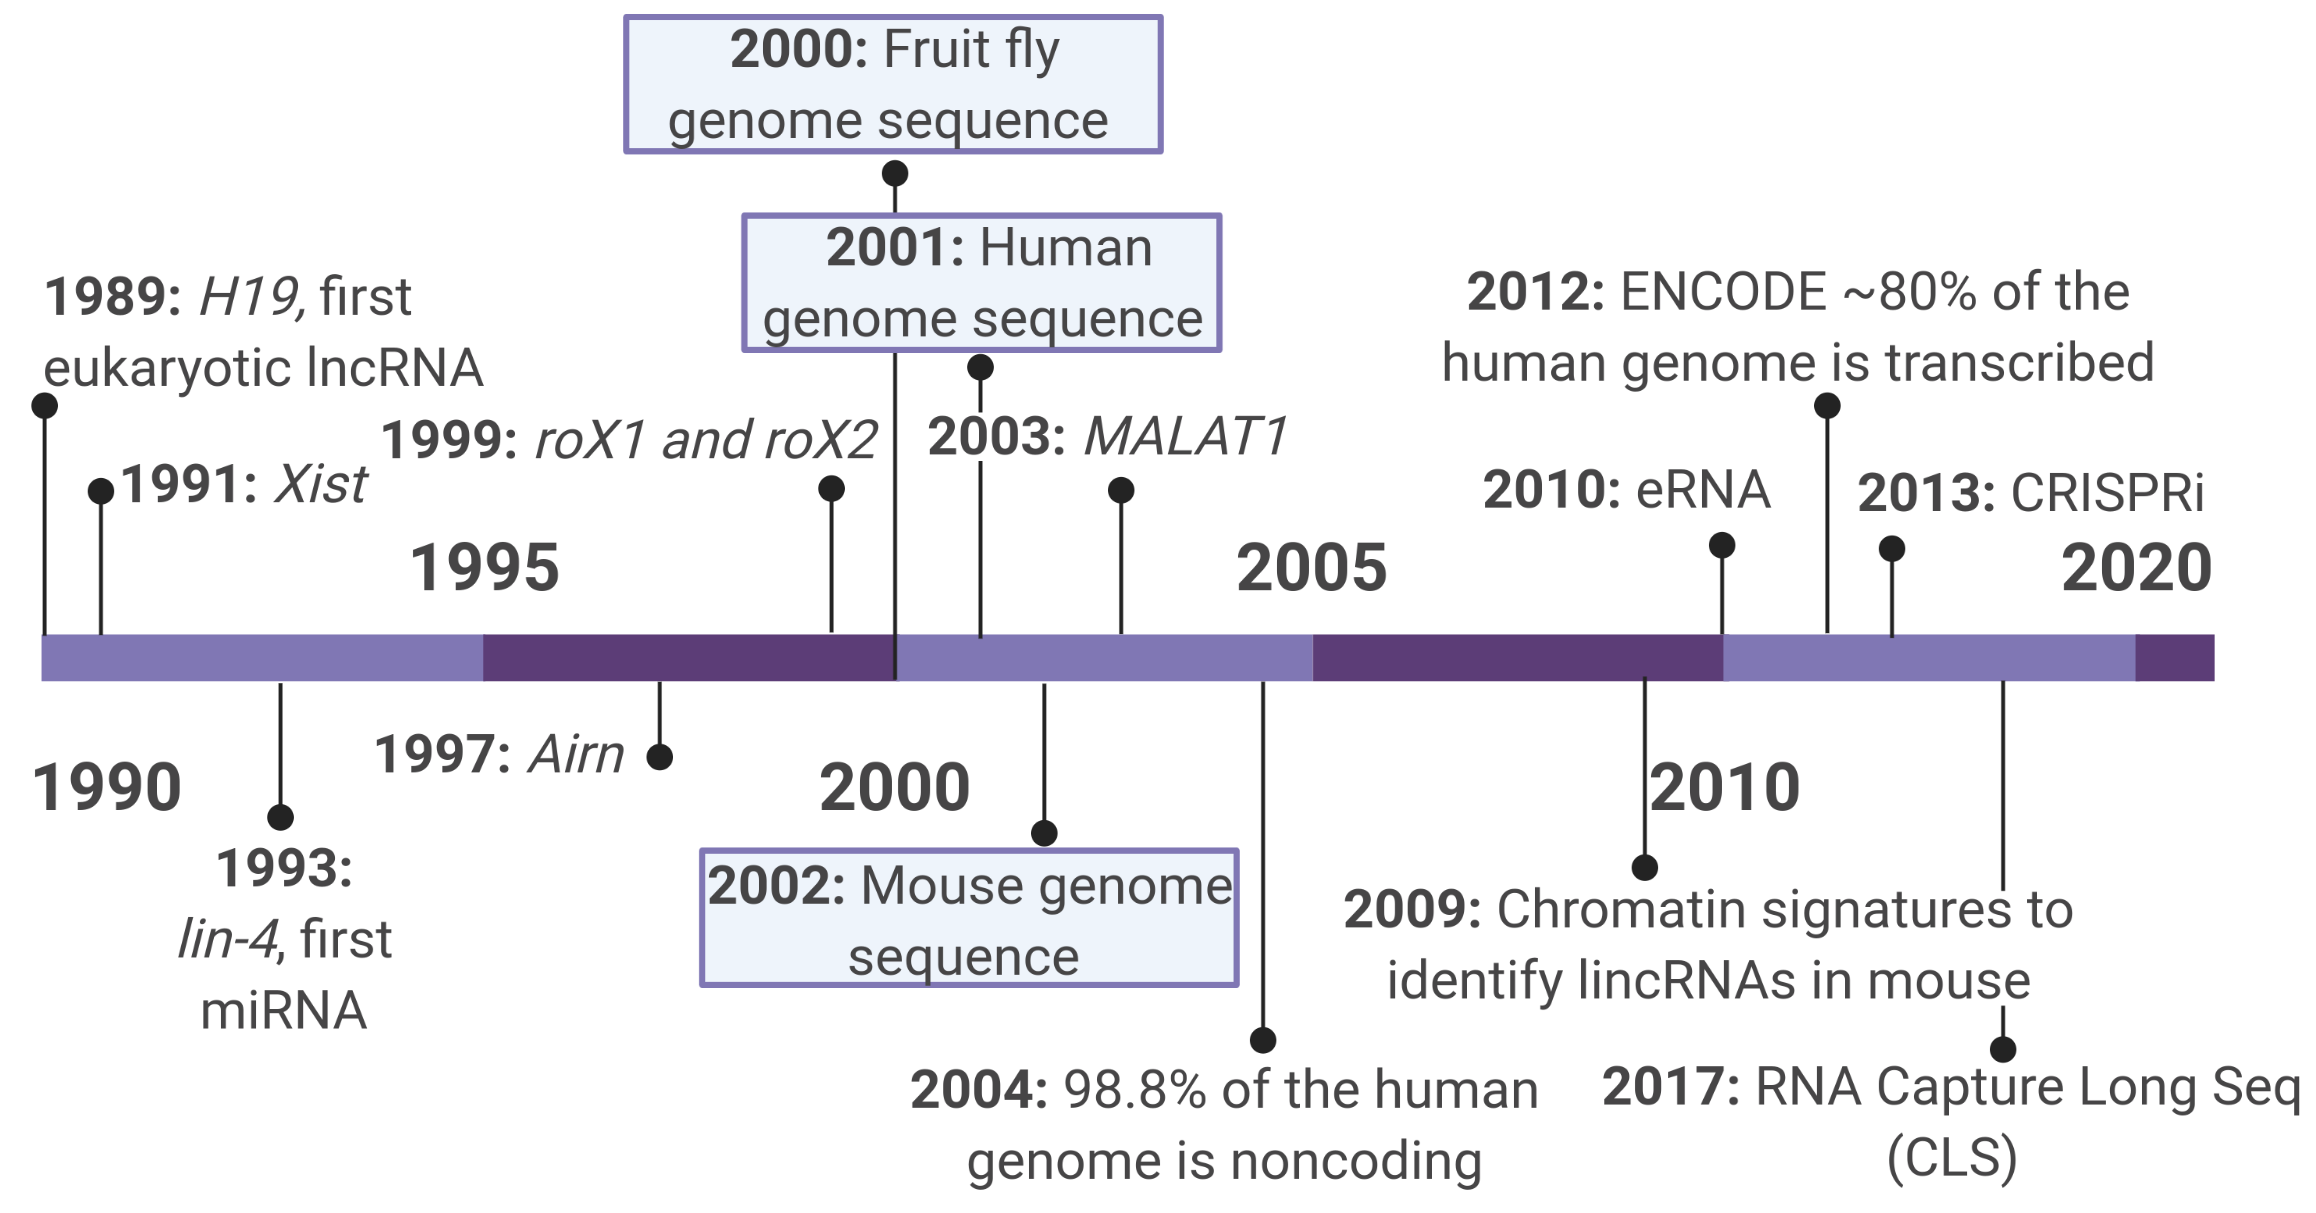
\includegraphics[width=0.9\textwidth]{img/introduction/lncRNA_timeline.png}
  \caption[LncRNA discoveries timeline]{\textbf{LncRNA discoveries timeline}. Main discoveries in noncoding RNAs, in particular lncRNAs.}
  \label{fig:lncRNA-time-line}
\end{figure}

\clearpage

\subsection{Long noncoding RNAs: a building block of biological processes}
\label{subsec:lncRNA_building_block}

Based on lncRNAs genomic positions relative to neighboring PCGs, lncRNAs can be classified as intergenic, genic exonic, or genic intronic if lncRNA loci come from an intergenic region, overlaps a protein-coding exon, or intron,\autocite{wucher_2017} respectively. LncRNAs are highly abundant in many organisms,\autocite{frankish_2021_gencode,thurmond_2019_flybase} such as humans (17,948 genes and 48,741 transcripts), mice (13,186 genes and 18,833 transcripts), and fruit flies (2,545 genes and 3,047 transcripts; see \autoref{fig:num-lncRNAs}), but other lncRNA annotations such as NONCODE\autocite{zhao_2021_noncodev6} estimates 96,411, 87,890, and 15,543 lncRNA genes for human, mouse, and fruit fly, respectively. 

\begin{figure}[!htb]
  \centering
  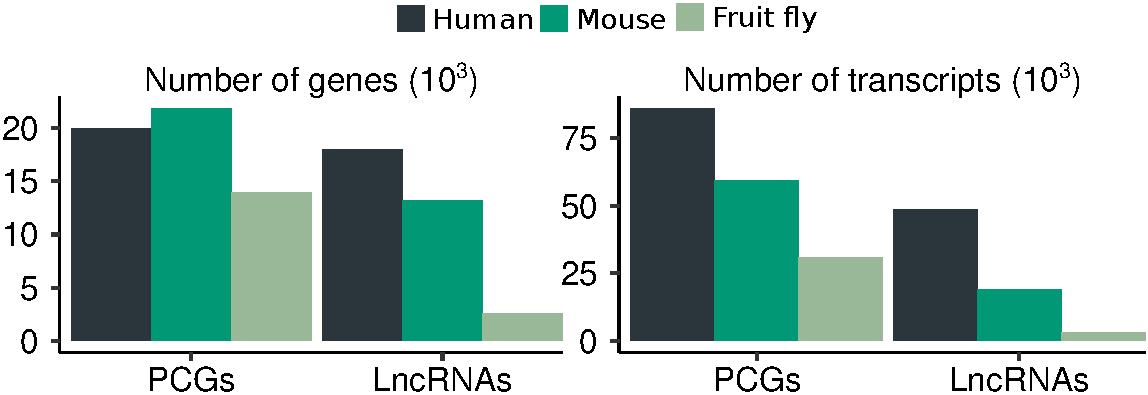
\includegraphics[scale=0.57]{plots/introduction/num.genes.transcripts.pdf}
  \caption[Statistics in the human, mouse and fruit fly genomes]{\textbf{Statistics in the human, mouse and fruit fly genomes}. Shown are the gene (left) and transcript (right) numbers for the PCG (left) and lncRNA (right) gene types. Inspired by.\autocite{derrien_2012_gencode}}
  \label{fig:num-lncRNAs}
\end{figure}

Mouse number of lncRNAs is mildly different from the human genome, however, it is unclear how much of this difference is biologically related rather than by the more mature status of the human genome annotation (\autoref{fig:num-lncRNAs}). For fruit fly \textit{Drosophila melanogaster} (\textit{D. melanogaster}) differences in the number of lncRNAs can be explained for the smaller \textit{Drosophila} genome with approximately 120 megabases, compared to the human and mouse genomes with 3,100 and 2,700 megabases,\autocite{adams_2000_dme_genome} respectively. Moreover, fewer differences for PCGs are observed among the human, mouse and fruit fly genomes, prompting the notion that PCGs are better annotated and conserved. 

There are at least three factors that make lncRNAs challenging to study. First, lncRNAs are poorly expressed compared to PCGs, meaning that lncRNA transcripts are underrepresented in any transcriptomic analysis, such as RNA sequencing (RNA-seq), expressed sequence tags (EST), tiling microarrays, and cap analysis of gene expression (CAGE) data.\autocite{uszczynska2018,derrien_2012_gencode} Second, lncRNAs show tissue-specific and condition-specific expression patterns, making it challenging to compare to other expression datasets.\autocite{djebali_2012_landscape,kopp_2018_functional} Third, lncRNAs tend to have little primary sequence conservation, meaning that ortholog and paralog analyses are challenging to implement.\autocite{zhao_2021_noncodev6,frankish_2021_gencode} See \autoref{tab:lncRNA_features} for further lncRNA and PCG comparisons. 

\begin{table}[!htb]
  \caption[Comparison of lncRNA and PCG features]{\textbf{Comparison of lncRNA and PCG features}. Only the longest transcript for each gene was considered; using the following gene annotations: the GENCODE Human, GENCODE Mouse, and/or Flybase reference annotations, versions: 37, M26, and r6.29, respectively (release: 2021).}
  \begin{scriptsize}
    \begin{tabulary}{0.65\linewidth}{cccc}
      \textbf{Feature} & \textbf{LncRNA} & \textbf{PCG} & \textbf{Reference} \\ \hline
      H3K4me1 & Low & Low & \autocite{jarroux_2017_history}  \\
      H3K4me3 & High & High & \autocite{jarroux_2017_history} \\
      H3K36me3 & Moderate/high & High & \autocite{jarroux_2017_history} \\
      H3K27ac & High & Low & \autocite{jarroux_2017_history} \\ \hline
      \multirow{4}*{\shortstack{Subcellular\\location}} & \multirow{4}*{\shortstack{Nucleus\\Cytosol\\Mitochondria\\Other organelles, \textit{e.g.} exosomes}} & \multirow{4}*{Cytosol} & \multirow{4}*{\autocite{statello_2021_lncRNA_reg}} \\ \\ \\ \\ \hline
      \multirow{3}*{\shortstack{Transcript\\length}} & \multirow{3}*{\shortstack{Human: 714 bp median\\ Mouse: 1087 bp median\\ Fruit fly: 646 bp median}} & \multirow{3}*{\shortstack{Human: $\sim$2.7 Kb median\\ Mouse: $\sim$2.5 Kb median\\ Fruit fly: $\sim$1.6 Kb median}} & \multirow{3}*{\shortstack{\autocite{frankish_2021_gencode}\\ \autocite{frankish_2021_gencode}\\\autocite{thurmond_2019_flybase}}} \\ \\ \\ \hline
      \multirow{2}*{\shortstack{RNA\\stability}} & \multirow{2}*{\shortstack{Variable, overall lower than PCG\\ Highly unstable: eRNA}} & \multirow{2}*{Variable} & \multirow{2}*{\autocite{jarroux_2017_history}} \\ \\
    \end{tabulary}
  \end{scriptsize}
  \label{tab:lncRNA_features}
\end{table}

In contrast with PCGs and short noncoding RNAs, the vast majority of lncRNAs functions remain enigmatic. LncRNA function has been subject of controversy, with few hundreds (or $\le$ 1\%) of experimentally validated or disease-associated lncRNAs.\autocite{uszczynska2018} Suggesting that lncRNA mere existence or production does not automatically imply functionality. Nevertheless, it is well documented that a growing number of lncRNAs are associated with relevant biological processes.\autocite{statello_2021_lncRNA_reg,kopp_2018_functional,li_2019_insights} Additionally, lncRNAs are predominantly localized in the nucleus and several lncRNAs control the expression of nearby genes (\textit{cis-acting lncRNAs}) by affecting their transcription and chromatin features. Other several lncRNAs function away from their loci (\textit{trans-acting lncRNAs}); their functions can be structural, involvement in signaling pathways, and regulation of PCGs including splicing and translation.

Consequently, lncRNAs interact with several paramount cellular functions that are of great importance, and alteration of their expression is inherent to numerous diseases such as neuronal disorders, hematopoiesis and immune response, cancer, etc. Thus, lncRNAs constitute a major gene class and unraveling their function will constitute a better understanding of our genome. 

\subsubsection{LncRNA conservation}
\label{subsubsec:conservation_lncRNAs}

Comparative analyses of genes across species can be a powerful tool for understanding their functions and action modes. For instance, the miRNA \textit{let-7} is conserved from humans to nematodes.\autocite{pasquinelli_2000_let} Comparative analyses require two main inputs: sets of genes or genomes that can be compared, and bioinformatic tools for evaluating the conservation. Applying comparative analyses to lncRNAs is challenging for two main reasons. First, only a few lncRNAs had been annotated in species other than human, mouse, and fruit fly. Second, lncRNAs lack long conserved sequences or regions with strong conserved structures, which are important features for conservation algorithms. Consequently, lncRNA loci from various species can be compared in the three following levels:

\begin{enumerate}
\item \textbf{Primary sequence conservation:} The first approach is to apply whole-genome multiple alignments (\textit{e.g.} those available in the \textit{UCSC} genome browser) or directly align the query lncRNA with lncRNA databases from other species using BLAST/BLAT or other alignment tools. Sequence conservation results demonstrated that lncRNA exons are less conserved than PCG exons.\autocite{necsulea_2014_evolution,haerty_2013_mutations} Interestingly, lncRNA exons on average are more conserved than PCG introns and random intergenic sequences.\autocite{cabili_2011_integrative,marques_2009_catalogues} However, there are two main drawbacks of using multiple alignments, as shown in \autoref{tab:lncRNA_features} the length of lncRNAs are shorter than PCGs, and the violation of the key assumption that lncRNA exons in one species align to lncRNA exons in the other species, in many cases lncRNA loci are homologous to non-conserved sequences in the other species.\autocite{necsulea_2014_evolution,washietl_2014_evolutionary}
  
\item \textbf{Structure conservation:} when comparing lncRNAs across more-distant species, sequence conservation might not be the best approach. An open debate is whether secondary structure plays an important role in lncRNA biology, as it does in short noncoding RNAs\autocite{ulitsky_2018_interactions} (such as miRNA, tRNA, etc.). Two observations support the secondary structure importance, the rapid rate of lncRNA evolution and lncRNA ability to fold into secondary structures, many of which are stable, nevertheless forming secondary structures \textit{per se} does not imply function. A successful usage of structure conservation is the detection of distant homologs on lncRNAs \textit{roX1} and \textit{roX2} in \textit{Drosophila} species\autocite{quinn_2016_rapid} (\autoref{tab:lncRNA-conserved}). Quinn \textit{et al.} identified 43 new \textit{roX} orthologs in diverse \textit{Drosophila} species across $\sim$40 million years of evolution distance despite limited sequence similarity. In Pegueroles \textit{et al.} study in 4  nematode species, a higher number of lncRNA orthologs were identified using secondary structures.\autocite{pegueroles_2019_synteny} Unfortunately, the currently available secondary structure predicting tools are not accurate enough for long sequences as lncRNAs,\autocite{novikova_2013_3s} thus prediction should be considered with caution. Additionally, there is no correlation between the amount of secondary structure and overall sequence conservation.\autocite{managadze_2011_negative, yang_2015_human}

\item \textbf{Positional conservation:} it has been proposed that in some cases, lncRNA function acts through transcription \textit{per se} instead of transcript displaying a function for itself.\autocite{kopp_2018_functional,pelechano_2013,statello_2021_lncRNA_reg} For instance in mice, one of the functions of the lncRNA \textit{Airn} (a genic-intronic lncRNA overlapping the PCG \textit{Igf2r}) can be explained for its position and not \textit{Airn} transcript itself, repressing \textit{Igf2r} by both transcription interference and DNA methylation.\autocite{pelechano_2013,schertzer_2019_airn,santoro_2013_airn} In such lncRNAs, we would expect that the position of the region that is transcribed would be conserved, whereas the exon positions would evolve neutrally. The lncRNA \textit{PVT1} can serve as an example of transcribed region conservation, \textit{PVT1} shows deep positional conservation (\autoref{tab:lncRNA-conserved}) but the transcript length and exon-intron architecture evolved rapidly.\autocite{hezroni_2015_principles} The \textit{LincOFinder} pipeline added its own worth by uncovering 16 homologous lncRNAs between very evolutionary distant species, humans and amphioxus by position conservation.\autocite{herrera_2019_microsyntenic} Although, positional conservation has shown promising results unveiling homologous lncRNAs, its approach is only applied to lincRNAs, leaving aside overlapping lncRNAs. Moreover, positional conservation deeply relies on orthologous PCGs discarding lincRNAs within low coding-gene content. 
\end{enumerate}

Given the different levels of lncRNA conservation based on probability of conserved functionality, proximity to PCGs, overlap with transposable elements, tissue specificity, and expression levels; it has been proposed three levels of lncRNA classification: class I, class II, and class III.\autocite{ulitsky_2016_evolution} In class I, lncRNA exon-intron structure and multiple sequences along the lncRNA locus are conserved across species, lncRNAs: \textit{MALAT1}, \textit{NEAT1}, and \textit{NORAD} can be classified as class I (\autoref{tab:lncRNA-conserved}). In class II, lncRNAs are those in which the act of transcription and some RNA elements are conserved, whereas the majority of lncRNA locus experienced drastic changes in exon-intron structure and length, \textit{lnc-ONECUT1} (\textit{LINC02490}) can serve as a class II example (\autoref{tab:lncRNA-conserved}). In class III, lncRNAs show promoter sequence conservation and the act of transcription on the specific region, for example, the lncRNA \textit{FENDRR} display promoter conservation. 

\begin{table}[!htb]
  \caption[Example of conserved lncRNAs]{\textbf{Example of conserved lncRNAs}. e-i$^*$= exon-intron structure.}
  \begin{scriptsize}
    \begin{tabulary}{0.65\linewidth}{lll}
      \textbf{LncRNA} & \textbf{Conservation level} & \textbf{Mechanism} \\ \hline
      \textit{roX1}-\textit{roX2}\autocite{flintoft_2013_rox} & Conserved in \textit{Drosophila} species & Fruit fly dosage compensation \\
      \textit{PVT1}\autocite{hezroni_2015_principles} & Deep positional conservation & Function as an oncogene in different cancers \\
      \textit{MALAT1}\autocite{statello_2021_lncRNA_reg} & Multiple conserved sequence and e-i$^*$ structure & Involved in structural functions \\
      \textit{NEAT1}\autocite{ulitsky_2016_evolution,statello_2021_lncRNA_reg} & Multiple conserved sequence and e-i$^*$ structure & A scaffold lncRNA of paraspeckles \\
      \textit{NORAD}\autocite{ulitsky_2016_evolution} & Multiple conserved sequence and e-i$^*$ structure & Promotes PCG stability for genome integrity\\
      \textit{lnc-ONECUT1}\autocite{ulitsky_2016_evolution} & Transcription and some elements are conserved & NA \\
      \textit{FENDRR}\autocite{ulitsky_2016_evolution} & Transcription and promoters are conserved & Is an essential regulator of heart \\
    \end{tabulary}
  \end{scriptsize}
  \label{tab:lncRNA-conserved}
\end{table}

\subsubsection{Small Open Reading Frames (smORFs) within lncRNA genes}
\label{subsubsec:smORFS}

By definition, lncRNAs lack coding potential. Surprisingly, 98\% of annotated lncRNAs contain at least one small Open Reading Frame (smORF) in the human, mouse and fruit fly genomes with a median of six smORFs per lncRNA.\autocite{couso_2017_smORF} In consequence, Couso \textit{et al.} results challenge the current definition of lncRNAs.

smORFs contain 10 to 100 codons, and millions of smORF sequences are found in eukaryotic genomes.\autocite{couso_2017_smORF,andrews_2014_smorf} The putative function of these peptides is, however, often neglected and the genes that encode them remain listed as noncoding. The \textit{tal} gene can be used as an example, which was previously annotated as noncoding, \textit{tal} gene encodes 4 small peptides of 11 amino acids.\autocite{couso_2017_smORF} Nevertheless, examples of small-functional-peptides have been described functioning as regulators of membrane-associated proteins, or as components of ancient protein complexes.\autocite{pueyo_2016_peptides}

There are six smORF classes based on their RNA type, median codon size, translation rate, coding features, and function. smORFs within lncRNAs represent the third most abundant class of smORFs with a low translation efficiency.\autocite{couso_2017_smORF} These results highlight our poor lncRNA definition, and the need for more classification parameters in addition to length cutoff.  

\clearpage

\section{LncRNA roles and mechanisms of action}
\label{sec:lncRNA-function}

LncRNA roles and mechanisms of action, to this day, still struggle to keep pace with the ever-growing lncRNA catalogs: of the thousands of currently discovered lncRNA loci, less than 500 have robustly assigned cellular function.\autocite{quek_2015_lncrnadb} Functional lncRNAs can be classified as "\textit{cis-acting lncRNAs}", when they influence the expression, splicing and/or chromatin state of nearby genes, or "\textit{trans-acting lncRNAs}", which act far from their locus.\autocite{kopp_2018_functional} Based on our current understanding, functional lncRNAs can influence gene expression at three main levels: \textbf{1)} chromatin regulation, \textbf{2)} transcriptional regulation, and \textbf{3)} post-transcriptional regulation.\autocite{statello_2021_lncRNA_reg,li_2019_insights}

\subsection{Chromatin regulation}
\label{sub-sec:lncRNA_chromatin_reg}

Two famous lncRNAs \textit{Xist} and \textit{Airn} involved in chromatin regulation were discovered before the Human Genome Project (see \autoref{fig:lncRNA-time-line}). \textit{Xist} involved in mammalian dosage compensation, and \textit{Airn} antisense to the imprinted \textit{Igf2r} gene.\autocite{loda_2019_xist,santoro_2013_airn}

\textit{Airn} was uncovered by Wutz \textit{et al.} as the first lncRNA in regulating the imprinted expression of neighboring PCGs.\autocite{wutz_1997_imprinted} \textit{Airn} is an intronic antisense lncRNA overlapping the PCG \textit{Igf2r}. Additionally, \textit{Airn} functions as \textit{trans-acting lncRNA} placing on the promoters of two distal imprinted target genes, \textit{Slc22a2} and \textit{Slc22a3}. Once there \textit{Airn} recruits PRC2, which catalyzes H3K27me3 leading to gene silencing in mouse stem cells.\autocite{schertzer_2019_airn}

As these two early unveiled lncRNAs were implicated in chromatin regulation, their discovery raised expectations that chromatin regulation might be a common feature of lncRNAs. Since then, several lncRNAs have been associated in displaying direct interaction with chromatin \textit{in cis} and \textit{in trans}, in the recruitment of chromatin modifiers, and acting as a decoy of chromatin modifiers. (See \autoref{tab:lncRNA_chromatin_reg} to have a summarized view of lncRNAs involved in chromatin regulation). 

\begin{table}[!htb]
  \caption[LncRNAs involved in chromatin regulation]{\textbf{LncRNAs involved in chromatin regulation}}
  \begin{scriptsize}
    \begin{tabulary}{0.65\linewidth}{llll}
      \textbf{LncRNA} & \textbf{Interacting with} & \textbf{Mechanism} & \textbf{Sequence features} \\ \hline
      \textit{Xist}\autocite{loda_2019_xist} & PRC2,YY1,hnRNPK,etc. & Silences X-linked genes & Long range interaction \\
      \textit{Airn}\autocite{schertzer_2019_airn} & PRC2 & Silences \textit{Slc22a2} and \textit{Slc22a3} genes & NA \\
      \textit{TARID}\autocite{arab_2019_gadd45a} & \textit{GADD45A} & Forms R-loops and recruits \textit{GADD45A} & Interacts with GC-rich seq. \\
      \textit{ANRIL}\autocite{holdt_2013_anril} & PRC1 and PRC2 & Regulate distal genes \textit{in trans} & \textit{Alu} retroelements motifs \\
      \textit{HOTTIP}\autocite{luo_2019_hottip} & \textit{WDR5}-\textit{MLL} & Activates HOXA genes & NA \\
      \textit{lncPRESS1}\autocite{jain_2016_lncpress1} & \textit{SIRT6} & Functions as \textit{SIRT6} decoy & NA \\
      \textit{APOLO}\autocite{mas_2020_apolo} & \textit{LHP1} & Functions as \textit{LHP1} decoy & Two TTCTTC boxes \\
    \end{tabulary}
  \end{scriptsize}
  \label{tab:lncRNA_chromatin_reg}
\end{table}

\subsubsection{Direct interaction with chromatin}
\label{sub-sub-sec:direct_interaction_chr}

Dueva \textit{et al.} conclusions that the negative charge of RNA can neutralize the positively charged histone tails and numerous lncRNAs localized in the chromatin where lncRNAs can interact with proteins, suggest a rapid switch of gene expression.\autocite{dueva_2019_neutralization} The well-studied lncRNAs \textit{Xist} and \textit{Airn} can serve as examples of lncRNAs with direct interaction with chromatin acting \textit{in cis} and \textit{in trans}, respectively (see \nameref{subsub:early_lncRNA_discoveries} for further \textit{Xist} mechanistic details).\autocite{loda_2019_xist,schertzer_2019_airn}

Moreover, lncRNAs can form RNA-DNA hybrids such as R-loops, by interacting with DNA. The lncRNA \textit{TARID} mechanism of action is explained through R-loops with \textit{GADD45A} locus, which drives the methylation of the \textit{TCF21} promoter and consequently silences \textit{TCF21} expression.\autocite{arab_2019_gadd45a} Holdt \textit{et al.} work reported that the lncRNA \textit{ANRIL} interacts with chromatin as a \textit{trans-acting lncRNA} through \textit{Alu} motifs, which drives \textit{ANRIL} recruitment of PCR1 and PCR2 to distal genes leading to increased cell proliferation, increased cell adhesion and decreased apoptosis.\autocite{holdt_2013_anril}

\subsubsection{Recruitment of chromatin modifiers}
\label{sub-sub-sec:recruitment_chromation_modifiers}

LncRNAs can interact with chromatin modifiers and recruit them to target PCG regulatory elements to activate or inactivate their locus expression \textit{in cis}, or \textit{in trans}. The lncRNA \textit{HOTTIP} is one of the several lncRNAs that regulate the \textit{HOXA} gene cluster, \textit{HOTTIP} is localized upstream of the \textit{HOXA} cluster, and \textit{HOTTIP} expression contributes to the maintenance of chromatin organization in \textit{HOXA} region.\autocite{wang_2011_hottip}

\textit{HOTTIP} recruits the mixed-lineage leukemia (MLL; also known as KMT2A) complex, which is a chromatin modifier, to activate the expression of the \textit{HOXA} genes through H3K4me3 chromatin mark and playing as a notable regulator of mouse hematopoietic stem cells.\autocite{luo_2019_hottip}

\subsubsection{Acting as a decoy of chromatin modifiers}
\label{sub-sub-sec:decoy_lncRNA}

In addition to interacting with chromatin and recruitment of chromatin modifiers, lncRNAs may function as decoys of chromatin modifiers by sequestering them from the DNA regulatory regions of target genes. For example, the lncRNA \textit{lncPRESS1} acts as a decoy of \textit{SIRT6} chromatin modifier.\autocite{jain_2016_lncpress1}

\textit{LncPRESS1} supports the pluripotency of human embryonic stem cells by sequestering \textit{SIRT6} from the promoters of numerous pluripotency genes by maintaining active H3K56ac and H3K9ac chromatin marks. During p53-mediated differentiation or \textit{lncPRESS1} depletion, \textit{SIRT6} localizes to the chromatin and inhibits the expression of pluripotency genes.\autocite{jain_2016_lncpress1}

The \textit{APOLO} gene is another lncRNA that functions as a decoy of chromatin modifiers.\autocite{mas_2020_apolo} In \textit{Arabidopsis thaliana} (\textit{A. thaliana}), \textit{APOLO} acts as a decoy of \textit{LHP1} during auxin response. Normally, \textit{APOLO} and auxin target genes are silenced by H3K27me3 and the presence of the Polycomb factor-like heterochromatin 1 (\textit{LHP1}). Then, in response to auxin \textit{APOLO} is expressed and acts \textit{in trans} to target its target gene promoters forming R-loops and acting as a decoy of \textit{LHP1}, thereby allowing target-gene expression.\autocite{ariel_2020_apolo}

\subsection{Transcriptional regulation}
\label{sub-sec:lncRNA_transcriptional_reg}

The non-random genomic arrangement of lncRNAs throughout genomes could represent a key determinant for lncRNAs to regulate PCGs transcription. Moreover, Seila \textit{et al.} reported antisense and bidirectional lncRNA transcription to be evolutionarily conserved, this could represent an evolutionary adaptation of genes to regulating their own transcription in a context-specific manner.\autocite{seila_2008_divergent}

Under Luo \textit{et al.} results, we analyzed lincRNAs with a locus-locus distance from their closest neighboring PCG lower of 5 Kb for the human and mouse genomes, and 1 Kb for the fruit fly genome. Our observations are in agreement with Luo \textit{et al.} study, where divergent lincRNAs are the most common lincRNA class in the human, mouse and fruitlfy genomes\autocite{luo_2016_divergent} (\autoref{fig:statistics_lincRNA}). In addition, we observed fewer differences between the divergent lincRNA class and the rest of the lincRNA classes within the fruit fly genome; this could explained by lower levels of bidirectionality in \textit{D. melanogaster}.\autocite{core_2012_defining} Consequently, these non-random genomic arrangements of divergent lincRNAs suggest lncRNAs play a pivotal role in regulating nearby PCGs transcription.

\begin{figure}[!htb]
  \centering
  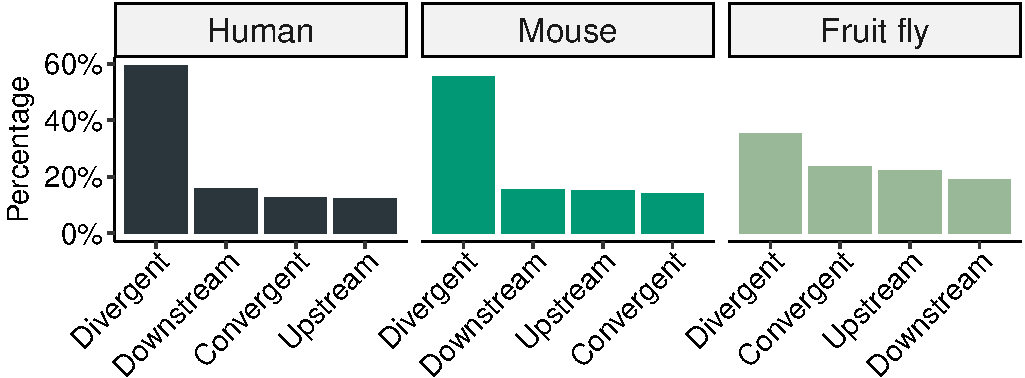
\includegraphics[scale=0.57]{plots/introduction/lincRNA.subtypes.pdf}
  \caption[LincRNA classification for the human, mouse and fruit fly genomes.]{\textbf{LincRNA classification for the human, mouse and fruit fly genomes.}. Percentage of lincRNA classification for genes with a distance < 5 Kb between lincRNA locus and the closest neighboring PCG for human and mouse, and < 1 Kb for fruit fly. Inspired by.\autocite{luo_2016_divergent}}
  \label{fig:statistics_lincRNA}
\end{figure}

LncRNA regulates PCG transcription by two main mechanisms, and non-mutually exclusive \textbf{1)} transcript-dependent: the lncRNA transcript for itself can regulate PCG loci (\textit{in cis} or \textit{in trans}), or \textbf{2)} transcript-independent: the act of transcription of the lncRNA can generate a steric impediment or chromatin state that influence the expression of nearby genes.   

\subsubsection{Transcript-dependent regulation}
\label{subsub-sec:trans-dep-reg}

The \textit{cis-acting} lncRNA \textit{ANRASSF1} is an antisense genic-exonic of the PCG \textit{RASSF1}, which is a tumor suppressor gene in different cancers. The lncRNA \textit{ANRASSF1} can serve as an example of transcript-dependent regulation, \textit{ANRASSF1} is transcribed from the opposite strand of the \textit{RASSF1} locus and is responsible for recruiting PRC2 to the \textit{RASSF1} promoter region, leading to the H3K27me3 repressive marks. \textit{ANRASSF1} transcript has a function for itself, forming an RNA/DNA hybrid and recruiting PRC2 to the \textit{RASSF1} promoter.\autocite{statello_2021_lncRNA_reg}

In \textit{A. thaliana}, the \textit{cis-acting} lncRNA \textit{COOLAIR} is an antisense genic-exonic of the \textit{FLC} locus, which is a regulator of the transition to reproduction. \textit{COOLAIR} transcript is cold-induced and is involved in the epigenetic silencing of the PCG \textit{FLC} through changed H3K36me3/H3K27me3 dynamics. Cold strongly upregulates \textit{COOLAIR} transcript, which lingers at its site of transcription and coats the locus to promote PRC2-dependent H3K27me3 leading to \textit{FLC} silencing.\autocite{statello_2021_lncRNA_reg}

As a \textit{trans-acting} lncRNA with transcript functionality, we can highlight the lncRNA \textit{HOTAIR}. \textit{HOTAIR} is an antisense genic-intronic lncRNA of the \textit{HOXC} locus. \textit{HOX} transcription factors (TFs) encoded from four \textit{HOX} gene clusters (\textit{HOXA}, \textit{HOXB}, \textit{HOXC}, and \textit{HOXD}) are deeply conserved and involved in positional identity and differentiation.\autocite{carnesecchi_2018_hox,statello_2021_lncRNA_reg} \textit{HOTAIR} is required to maintain repressive chromatin marks at the distant \textit{HOXD} locus through interactions between \textit{HOTAIR} and components of PRC2.\autocite{kopp_2018_functional,pelechano_2013}  Depletion of \textit{HOTAIR} with small interfering RNAs (siRNAs) resulted in transcriptional activation of \textit{HOXD} genes with an associated decrease in the repressive chromatin mark H3K27me3.\autocite{statello_2021_lncRNA_reg}

\subsubsection{Transcript-independent regulation}
\label{subsub-sec:trans-indep-reg}

LncRNAs can suppress gene expression by interfering with the transcription machinery, which leads to alteration of the recruitment of TFs or Pol II at the inhibited promoter, alteration of histone modifications, and reduction of chromatin accessibility. Several transcript-independent mechanisms have been proposed (reviewed in \autocite{statello_2021_lncRNA_reg,kopp_2018_functional,pelechano_2013}), but in this thesis work we will analyze three main mechanisms: \textbf{1)} RNA polymerase collision, \textbf{2)} regulatory elements embedded within lncRNA loci, and \textbf{3)} the increasing roles of eRNAs.  

\paragraph{RNA polymerase collision}
\label{paragraph:rna_pol_coll}

LncRNA transcription can regulate neighboring PCG expression after transcriptional initiation by transcriptional interference that occurs co-transcriptionally. This mechanism can be mediated by direct RNA polymerase collision by "\textit{sitting-duck}" interference\footnote{When an elongating polymerase removes another that is already attached to a gene promoter.} or by one RNA polymerase acting as a "\textit{roadblock}" for other incoming elongating polymerase.\autocite{pelechano_2013} If a gene is simultaneously transcribed in both directions, this leads to RNA polymerase collision (\autoref{fig:transcriptional_reg}A).

Nonetheless, \textit{in vitro} phage polymerases that act in both directions are able to bypass each other; this is not the case for more complex bacterial or eukaryotic RNA polymerases.\autocite{hobson_2012_collision} Additionally, transcriptional interference by direct polymerase collision is most likely when two strong convergent genes are present, conversely, it is unlikely for two weak convergent genes.\autocite{pelechano_2013}

In \textit{D. melanogaster}, the lncRNA \textit{bsAS} (FlyBaseID=\textit{CR44811}) regulates its PCG by polymerase collision. \textit{bsAS} is an antisense genic-intronic of the PCG \textit{bs}, which is involved in wing development and formation.\autocite{nussbaumer_2000_bs} \textit{bsAS} is involved in the regulation of \textit{bs} isoform usage in flies in a tissue-specific manner, by the transcription of \textit{bsAS}.\autocite{perez_blister} Expression of \textit{bsAS} occurs specifically in wing intervein regions and impairs the transcription of the \textit{bs} long isoforms, thus promoting the expression of the short isoform. Pérez-Lluch \textit{et al.} proposed the RNA polymerase collision mechanism (\autoref{fig:transcriptional_reg}A) to explain the inhibition of the \textit{bs} long isoform. 

Furthermore, the lncRNAs \textit{Airn}\footnote{See \nameref{subsubsec:conservation_lncRNAs} for a detailed \textit{Airn} \textit{cis-acting} mechanism.} and \textit{Chaserr} mechanisms of action are explained by polymerase collision. \textit{Chaserr} is a conserved lncRNA and is located upstream of the \textit{Chd2} gene, which is a chromatin remodeler implicated in neurological disorders.\autocite{rom_2019_chaserr}

\paragraph{Regulatory elements embedded within lncRNA loci}
\label{paragraph:regulatory_within}

As described above, functional DNA elements within lncRNA loci can activate the expression of neighboring genes (\autoref{fig:transcriptional_reg}B). The lncRNA \textit{Bendr} regulates \textit{in cis} its neighboring gene, \textit{BEND4}, through the presence of enhancer elements in its locus. The enhancer element is activated by \textit{Bendr} transcription.\autocite{statello_2021_lncRNA_reg,engreitz_2016_local}

The lincRNA \textit{p21} provides another instructive example of regulatory elements within lncRNAs. \textit{p21} is a nuclear-localized transcript that neighbors the \textit{CDKN1A} gene in humans and mice. Genetic analyses of the lincRNA \textit{p21} uncovered that its locus contains \textit{cis-regulatory} DNA elements that modulate \textit{CDKN1A} expression.\autocite{statello_2021_lncRNA_reg} Other lncRNAs have been reported with similar roles in the activation of proximal enhancers,\autocite{engreitz_2016_local} such as the lncRNA \textit{Uph}.\autocite{anderson_2016_transcription}

\begin{figure}[!htb]
  \centering
  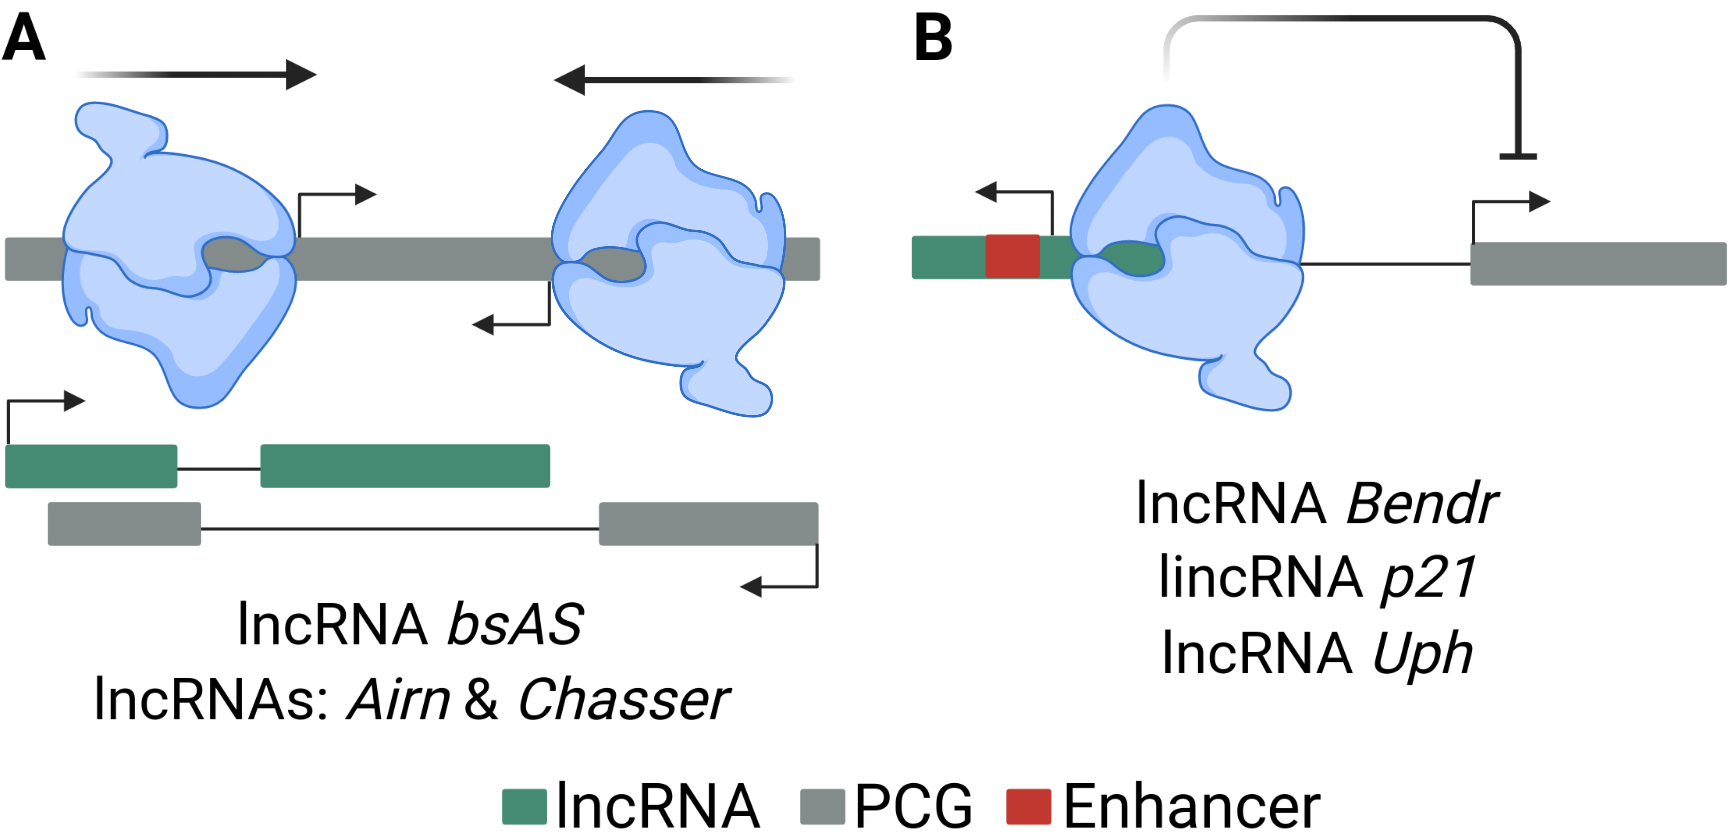
\includegraphics[width=0.7\textwidth]{img/introduction/transcriptional_reg.png}
  \caption[Transcript-independent mechanisms]{\textbf{Transcript-independent mechanisms}. \textbf{(A)} RNA polymerase collision. \textbf{(B)} Regulatory elements embedded within lncRNA loci.}
  \label{fig:transcriptional_reg}
\end{figure}

\paragraph{eRNAs}
\label{paragraph:eRNA}

Active enhancers can be transcribed into two main types of noncoding RNAs: eRNA and enhancer-associated lncRNAs (elncRNAs).\autocite{arnold_2020_diversity} The main distinction between eRNAs and elncRNAs is their genomic features. elncRNAs are mostly unidirectional, polyadenylated, spliced, longer (up to 4 Kb) and transcribed from higher-activity enhancers. By contrast, eRNAs are bidirectional capped transcripts, non-polyadenylated, unspliced, shorter (< 2 Kb), unstable and transcribed from H3K4me1 marked enhancers.\autocite{arnold_2020_diversity,statello_2021_lncRNA_reg,mikhaylichenko_2018_erna,syed_2021_heterogeneity} Moreover, the general features of eRNA and elncRNA are highly conserved from humans to flies.\autocite{mikhaylichenko_2018_erna}

The literature overall supports a model wherein eRNAs contribute to enhancer action by interacting with nuclear proteins to promote enhancer-promoter looping, and gene regulation.\autocite{arnold_2020_diversity,statello_2021_lncRNA_reg} For instance, the lncRNA \textit{eNRIP} is transcribed into an eRNA, which recruits cohesin to form enhancer-promoter looping. Thus, promoting contact between \textit{NRIP1} and \textit{TFF1} promoters leads to loci expression of these genes, this mechanism is regulated by estrogen receptor activation.\autocite{statello_2021_lncRNA_reg}

\subsection{Post-transcriptional regulation}
\label{sub-sec:lncRNA_post_trans_reg}

In addition to their roles in chromatin and transcriptional regulation, lncRNAs can act through their ability to establish interactions with proteins and nucleic acids regulating PCGs post-transcriptionally.\autocite{romero_2018_splicing,kopp_2018_functional} Here, we highlight a few of the many different modes lncRNA functions as post-transcriptional regulators, mainly focusing on: \textbf{1)} lncRNAs as a source of miRNAs and \textbf{2)} lncRNAs regulating PCG splicing. 

\begin{figure}[!htb]
  \centering
  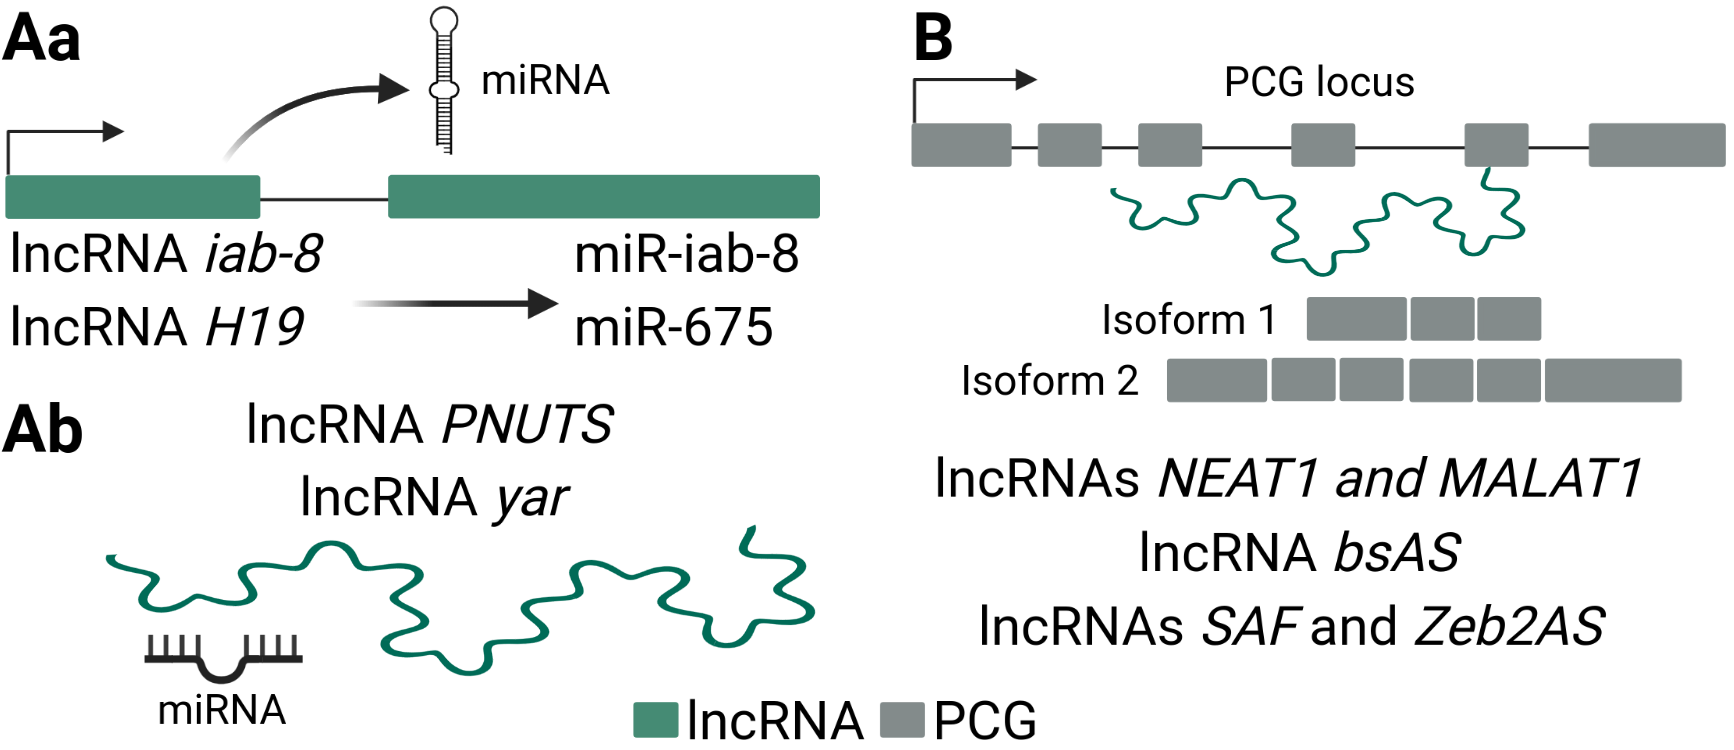
\includegraphics[width=0.74\textwidth]{img/introduction/post_transcriptional_reg.png}
  \caption[Post-transcriptional regulation of lncRNAs]{\textbf{Post-transcriptional regulation of lncRNAs}. \textbf{(Aa)} LncRNAs as a source of miRNAs. \textbf{(Ab)} LncRNAs acting as miRNA "\textit{sponges}". \textbf{(B)} LncRNAs regulating isoform usage.}
  \label{fig:post-trans-reg}
\end{figure}

\subsubsection{LncRNAs as a source of miRNAs}
\label{subsub-sec:lncRNA-miRNA}

miRNAs are short noncoding RNAs ($\sim$22 nucleotides), which play a relevant role in the post-transcriptional regulation of gene expression.\autocite{siomi_2010_mirna} In many cases, miRNAs are derived from the introns or exons of larger genes ("\textit{host}"). If the miRNA is processed from the host exonic sequence, the processing reaction typically leads to rapid exonucleolytic degradation of the host. By contrast, if the miRNA is processed from the host intronic sequence the host RNA stability is typically not affected.\autocite{ulitsky_2018_interactions}

In \textit{D. melanogaster}, the lncRNA \textit{iab-8} acts as a source of miRNAs. Once transcribed, lncRNA \textit{iab-8} is processed into three miRNAs transcripts that are collectively called miR-iab-8, these miRNAs are processed from lncRNA \textit{iab-8} intronic sequence. These miRNAs are known to target and downregulate the homeotic genes \textit{abd-A} and \textit{Ubx}, as well as their cofactors \textit{hth} and \textit{exd}.\autocite{garaulet_2014_homeotic} Knocking down lncRNA \textit{iab-8} expression results in male and female sterility.\autocite{maeda_2018_lncrna}

In mammals, several lncRNAs have been described as precursors of miRNAs. A well-studied case is the maternally-imprinted \textit{H19} locus. During skeletal muscle differentiation and regeneration in mice, the lncRNA \textit{H19} is processed into the miRNA miR-675, which is embedded in \textit{H19} first intron. This miRNA functions by directly downregulating the \textit{Smad} TF.\autocite{kallen_2013_h19} In parallel, \textit{H19} is highly present in fetal tissues, where it is found to be processed into miR-675, which limits placental growth by targeting, among others, the PCG \textit{Igf1r}.\autocite{keniry_2012_h19} 

\paragraph{LncRNAs acting as "\textit{sponge}" of miRNAs}
\label{paragraph:lncRNA_mi_sponge}

Some lncRNAs contain miRNA complementary sites that can regulate gene expression as competitive endogenous RNAs or "\textit{sponges}" of miRNAs, thereby reducing miRNA availability to target PCGs.\autocite{cesana_2011_long,salmena_2011_cerna}

For instance, the lncRNA \textit{PNUTS} serves as a miRNA sponge of the microRNA miR-205. In tumors, the pre-mRNA \textit{PNUTS} generates the lncRNA \textit{PNUTS} through alternative splicing, the lncRNA locus contains seven miR-205 binding sites, decreasing the availability of miR-205 to bind and suppress its target genes (\textit{ZEB1} and \textit{ZEB2}).\autocite{grelet_2017_pnuts} In \textit{D. melanogaster}, the lncRNA \textit{yar} contains $\sim$33 miRNA binding sites, its cytoplasmic location, and its incapacity to affect transcription of neighboring genes suggest \textit{yar} may function as a miRNA sponge\autocite{soshnev_2011_yar}. Although, the exact mechanism remains enigmatic.

\subsubsection{LncRNAs regulating pre-mRNA splicing}
\label{subsub-sec:lncRNA-isoform}

Recently, certain lncRNAs have been shown to play a crucial role in regulating pre-mRNA alternative splicing (AS) in response to several stimuli or diseases.\autocite{romero_2018_splicing,he_2019_lncRNA_splicing} The main mechanisms involving lncRNAs in AS modulation can be classified in two ways: \textbf{1)} lncRNAs interacting with splicing factors (SFs), and \textbf{2)} lncRNAs forming RNA-RNA duplexes with pre-mRNA molecules. 

\paragraph{LncRNAs interacting with splicing factors}
\label{paragraph:lncRNA_sf}

Using genome-wide screenings, the intergenic lncRNAs \textit{NEAT1} and \textit{MALAT1} (or \textit{NEAT2}) were among the first lncRNA loci implicated to interact with SFs in mouse and human cells.\autocite{romero_2018_splicing} \textit{NEAT1}\autocite{romero_2018_splicing,statello_2021_lncRNA_reg} is localized in paraspeckles\footnote{Paraspeckles: nuclear domains that control sequestration of related proteins.}, whereas \textit{MALAT1}\autocite{romero_2018_splicing,statello_2021_lncRNA_reg} is part of the polyadenylated component of nuclear speckles\footnote{Nuclear speckles: nuclear domains enriched in pre-mRNA splicing factors.}. More recently, more lncRNAs were reported to modulate PCG AS (\textit{e.g.} \textit{SAF}, \textit{GOMAFU}, and \textit{LINC01133}).

Serine-arginine-rich (SR) proteins are part of a conserved protein family involved in splicing.\autocite{romero_2018_splicing} SR proteins are commonly localized in the nucleus (although several of them are known to shuttle between the nucleus and the cytoplasm) and their function in splicing is linked to its phosphorylation status.\autocite{romero_2018_splicing}

During adipocyte differentiation, \textit{NEAT1} modulates the AS profile of the \textit{PPAR}$\gamma$ pre-mRNA into \textit{PPAR}$\gamma$\textit{-1} or \textit{PPAR}$\gamma$\textit{-2} isoforms. \textit{NEAT1} modulates \textit{SRp40} phosphorylation status by interacting with the \textit{Clk} kinase.\autocite{jiang_2009_akt2} Phosphorylated \textit{SRp40} promotes the processing of the \textit{PPAR}$\gamma$ pre-mRNA into the \textit{PPAR}$\gamma$\textit{-2} isoform. By contrast, the dephosphorylation of \textit{SRp40} promotes the \textit{PPAR}$\gamma$\textit{-1} isoform expression.\autocite{cooper_2014_neat1} \textit{PPAR}$\gamma$ encodes for the major TF implicated in adipocyte differentiation, in consequence \textit{NEAT1} modulation plays a relevant for cell viability and function. Additionally, \textit{NEAT1} depletion causes a decrease of \textit{PPAR}$\gamma$\textit{-1} and \textit{PPAR}$\gamma$\textit{-2} isoforms, in particular \textit{PPAR}$\gamma$\textit{-2} isoform.  

The lncRNA \textit{MALAT1} acts as an oncogene and its abnormal transcription is implicated in the development and progression of many cancers.\autocite{wang_2016_malat1,malakar_2017_malat1} Results in human cells demonstrate that \textit{MALAT1} regulates splicing by modulating SR splicing factors distribution and phosphorylation dynamics\autocite{tripathi_2010_malat1}. Depletion of \textit{MALAT1} enhances the dephosphorylated pool of SR proteins resulting in the mislocalization of speckle components and changes in AS of pre-mRNAs. The control of the levels of phosphorylated SR proteins impacts not only AS but also other SR post-transcriptional mechanisms, including RNA export, translation and nonsense-mediated decay.\autocite{romero_2018_splicing} The exact \textit{MALAT1} mechanism by which \textit{MALAT1} depletion alters the ratios of phosphorylated to dephosphorylated SR proteins in the cell remains elusive. However, it is possible \textit{MALAT1} regulates the action of the \textit{SRPK1} kinase and the \textit{PP1/2} phosphatase, which modify SR proteins.\autocite{romero_2018_splicing}

\paragraph{LncRNAs forming RNA-RNA duplexes with pre-mRNA molecules}
\label{paragraph:lncRNA_duplexes}

Overlapping lncRNAs in antisense represent 31.8\%, 27.1\% and 33.7\% of the human, mouse, and fruit fly genomes\autocite{frankish_2021_gencode,thurmond_2019_flybase}, respectively (overlapping in the coding and in the noncoding regions). Krystal \textit{et al.} detected RNA-RNA duplexes \textit{in vivo}, when the team was studying the oncogene \textit{N-myc} and its overlapping gene in antisense.\autocite{krystal_1990_rna-rna_duplex} Thus, it was postulated that RNA-RNA duplexes can modulate pre-mRNA splicing.  

In \textit{D. melanogaster}, the lncRNA \textit{bsAS} controls its PCG isoform usage\autocite{perez_blister} (see \nameref{paragraph:rna_pol_coll} for \textit{bsAS} mechanism). In mammals, the lncRNA \textit{SAF} is linked with apoptosis and cancer through the interaction between the \textit{FAS} receptor and its ligand.\autocite{} In human cell lines, \textit{SAF} is transcribed from the first intron of the \textit{FAS} locus. \textit{SAF} interacts with the exon 6 of the \textit{FAS} pre-mRNA, forming RNA-RNA duplexes. \textit{SAF} recruits the splicing factor \textit{SPF45} facilitating AS and exclusion of exon 6. The exclusion of exon 6 from the \textit{FAS} pre-mRNA leads to producing soluble \textit{FAS}, which lacks the transmembrane domain rendering cell less sensitive to \textit{FAS}-mediated apoptosis.\autocite{villamizar_2016_saf,villamizar_2016_fas}

Epithelial-mesenchymal transition (EMT) can be highlighted as another biological context where lncRNAs regulate PCG isoform usage through RNA-RNA duplexes. The genic-exonic \textit{Zeb2AS} overlaps in antisense with the \textit{Zeb2} locus. After EMT, the \textit{Snail} TF induces the transcription of the lncRNA \textit{Zeb2AS} in epithelial cells. A specific RNA-RNA duplex around the 5’ splice site of the 5’ UTR intron prevents the binding of the spliceosome.\autocite{beltran_2008_zeb2} Thus, favoring \textit{Zeb2} translation. In absence of \textit{Zeb2AS} transcription, the resulting mRNA contains a stable secondary structure before the first codon, which is able to block \textit{Zeb2} translation.\autocite{beltran_2008_zeb2,romero_2018_splicing}

\subsection{Conservation of lncRNA functions}
\label{paragraph:conservation_func}

The percentage of lncRNA conservation is increasingly regarded as a key feature in evaluating the impact of a studied lncRNA. If a lncRNA is involved in a human illness, it is relevant to know whether it can be studied in a model organism. Conversely, if a lncRNA is uncovered in a model organism, evidence of conservation is important to establishing relevance to human biology.

One paramount riddle is --if conserved lncRNAs also function in similar mechanisms in other species?-- Several studies have found that lncRNA tissue specificity as well as specific expression patterns, are generally highly conserved.\autocite{hezroni_2015_principles,ulitsky_2016_evolution} Thus, conserved lncRNA could act in similar contexts in different species. For instance, the lncRNA \textit{CARMEN} is required for cardiomyogenesis for both human and mouse cells,\autocite{ulitsky_2016_evolution} \textit{XIST} is required for X inactivation in humans and mice,\autocite{ulitsky_2016_evolution} and the lncRNA \textit{NEAT1} causes loss of paraspeckles across species (\autoref{tab:lncRNA-conserved-function}). 

\begin{table}[!htb]
  \caption[LncRNAs with conserved functions]{\textbf{LncRNAs with conserved functions}. e-i$^*$= exon-intron structure; lof$^*$= loss-of-function.}
  \begin{scriptsize}
    \begin{tabulary}{0.65\linewidth}{lll}
      \textbf{LncRNA} & \textbf{Conservation level} & \textbf{Mechanism} \\ \hline
      \textit{CARMEN}\autocite{ulitsky_2016_evolution} & Conserved lof$^*$ phenotype in mouse and human & Required for cardiomyogenesis \\
      \textit{XIST}\autocite{loda_2019_xist,ulitsky_2016_evolution} & Conserved across mammals & X inactivation in female mammals \\
      \textit{NEAT1}\autocite{ulitsky_2016_evolution,statello_2021_lncRNA_reg} & Multiple conserved sequence and e-i$^*$ structure & A scaffold lncRNA of paraspeckles \\
    \end{tabulary}
  \end{scriptsize}
  \label{tab:lncRNA-conserved-function}
\end{table}

\clearpage

\section[High-throughput screens to uncover functional lncRNAs]{High-throughput screens to uncover functional lncRNAs}
\label{sec:crispr}

After conducting a genome-wide transcriptome study comparing two biological conditions, we obtain a list of differentially expressed genes -- among them lncRNAs. However, this approach explains little or nothing about lncRNA biology and its mechanisms of action. Several reverse-genetics assays\autocite{liu_2017_crispri,Haswell_2021_crispri,liu_2020_crispri,cai_2020_crispri,liu_2020_crispri_glioma} have been successfully used to uncover lncRNA functions, searching for phenotypes after creating targeted mutations (\textit{e.g.} knockout and knockdown experiments)  in candidate loci. 

For PCGs a single insertion or deletion can abolish the PCG functionality. In contrast, for lncRNAs this approach does not apply due to our limited understanding of lncRNA functional domains. Consequently, other strategies are used including full-length deletion of lncRNA locus or deletion of lncRNA promoter regions.\autocite{perry_2016_functions,gao_2020_reverse_genetics} These constraints condition the loss-of-function approaches implemented in lncRNAs. Moreover, it is advisable to minimize the removal of DNA regions for lncRNA functional analyses.

Reverse-genetics methods can be broadly classified according to their targets, for instance acting directly at the lncRNA locus level (\textit{e.g.} DNA cleavage or local recruitment of silencing histone marks at the lncRNA TSS) or at the lncRNA transcript level (\textit{e.g.} RNA knockdown through RNAi).\autocite{gao_2020_reverse_genetics,morelli_2021_crispr} Acting at the RNA-level represents the most direct method for assessing lncRNA functionality without confounding factors caused by disruptions of DNA regulatory elements. RNA interference (RNAi) and antisense oligos (AOs) represent the most implemented methods for studying lncRNAs acting at the transcript level, with more than 1,500 studies unveiling lncRNA functionality in diverse cellular contexts\autocite{gao_2020_reverse_genetics} (see \autoref{tab:reverse-genetics}). RNAi and AOs knockdown their target lncRNAs through RISC and RNase H mediated mechanisms, respectively.\autocite{gao_2020_reverse_genetics,morelli_2021_crispr} The lncRNAs \textit{Neat1}, \textit{SPRY4-IT1}, \textit{DGCR5}, and other lncRNAs have been reported to show phenotypic consequences using RNAi and AOs methodologies.\autocite{clemson_2009_neat1,khaitan_2011_spry4-it1,meng_2018_dgcr5}

Nonetheless, RNAi and AOs methods present important disadvantages including the inability of genome-wide screens.\autocite{morelli_2021_crispr} Additionally, Stojic \textit{et al.} work demonstrated considerable off-target defects and sequence-dependent nature applying RNAi and AOs technologies within the HeLa cell line transcriptome.\autocite{stojic_2018_specificity} Moreover, RNAi incapacity to knockdown nuclear lncRNAs is a well-known drawback, hampering the analysis of a large fraction of lncRNAs.\autocite{stojic_2018_specificity,gao_2020_reverse_genetics,morelli_2021_crispr} Finally, these hurdles have paved the way for the usage of CRISPR-related systems.

\subsection{CRISPRi: genome-wide lncRNA screening}
\label{subsec:crispr-systems}

The bacterial Clustered Regularly Interspaced Short Palindromic Repeats (CRISPR)-Cas9 nuclease system is a highly adaptable technique, and has been used in many genome-wide editing studies.\autocite{cong_2013_crispr,mali_2013_crispr} Briefly, the CRISPR-Cas9 system works through the guiding of the Cas9 protein to a target sequence through a single guide RNA (sgRNA), the sgRNA directs the enzyme to bind DNA, where the nuclease induces a DNA double-strand break (DSB). Upon cleavage, the DNA repair machinery is recruited to the DSB, often inducing point mutations or frameshift mutations at the target locus to functionally knockout the PCG.\autocite{cong_2013_crispr,mali_2013_crispr}

CRISPR has been further modified for modulating locus expression without modifying the genomic sequence through the use of a nuclease-dead Cas9 (dCas9), which binds the target site without cleaving the DNA.\autocite{qi_2013_crispr} The CRISPR-dCas9 has been adapted for both gene inhibition (CRISPRi\autocite{gilbert_2013_crispri}) and activation (CRISPRa\autocite{maeder_2013_crispra,konermann_2015_crispra}). These inhibition and activation CRISPR-systems have been successfully applied in high-throughput screens in many different cells to improve the understanding and characterization of lncRNAs.\autocite{liu_2017_crispri,liu_2020_crispri_glioma,Haswell_2021_crispri} Further, the newly discovered Cas13 enzyme, which binds and modifies the RNA rather than the DNA, shows potential for high-throughput lncRNA analysis at the transcriptional level\autocite{guo_2021_cas13} (see \autoref{tab:reverse-genetics}).

CRISPRi is based on the use of dCas9 protein fused to the Krüppel-associated box (KRAB) transcriptional repression domain.\autocite{gilbert_2013_crispri} The CRISPRi system inhibits transcription in part through the dCas9 ability to sterically hinder RNA polymerase binding, and in part through the KRAB domain to place the repressive histone mark H3K9me3 at its target TSS\autocite{gilbert_2013_crispri,larson_2013_crispri,morelli_2021_crispr} (see \autoref{fig:crispri}). Gilbert \textit{et al.} demonstrated that the use of dCas9 and KRAB domain improved the knockdown of gene targets significantly compared to dCas9 alone.\autocite{gilbert_2013_crispri} In addition, the repression effect of CRISPRi is transient, and the effect is diminished until elimination at six to fourteen days after transfection.\autocite{nunez_2021_crispr} As shown in \autoref{fig:crispri}, the CRISPRi system deeply relies on the correct lncRNA TSS annotation, which in many times is not either complete or accurate leading to diminished CRISPRi effectiveness. 

\begin{figure}[!htb]
  \centering
  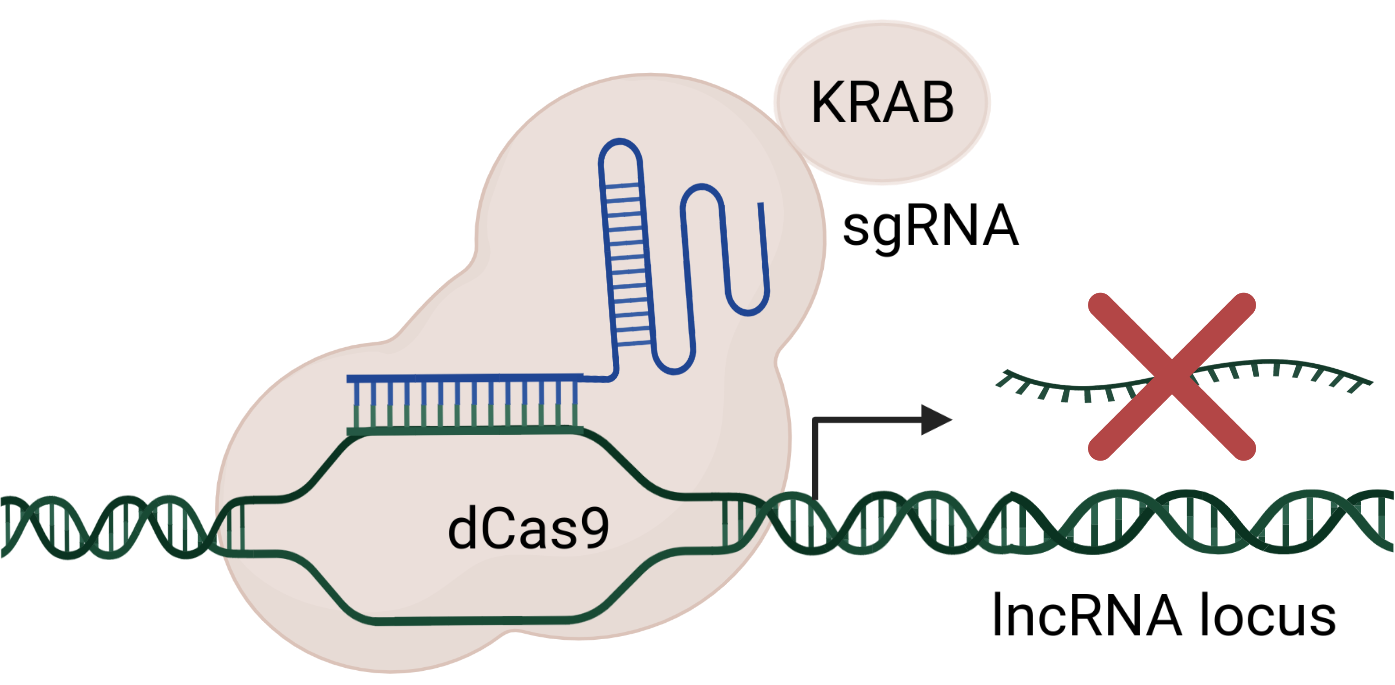
\includegraphics[width=0.55\textwidth]{img/introduction/CRISPRi.png}
  \caption[CRISPRi repression mechanism]{\textbf{CRISPRi repression mechanism}. Blue and green ribbons denote sgRNA and lncRNA locus, respectively.}
  \label{fig:crispri}
\end{figure}

Recently, additional repressive domains have been added to the dCas9-KRAB cassette to further improve the knockdown capabilities of the CRISPRi system. These additional repressive domains were selected by screening multiple domains from DNA-binding proteins. Notably, SIN3-interacting domain (SID), ZIM3, and methyl CpG binding protein 2 (MeCP2) were reported to improve the efficiency of repression by CRISPRi.\autocite{raffeiner_2020_sid_crispr,alerasool_2020_crispr_zim3} Moreover, for achieving long-term repression effects, the domains DNMT3A, DNMT3L, and Tet1 have been fused to dCas9, which are specifically designed to alter the DNA methylation states.\autocite{nunez_2021_crispr_epigenetics}

The CRISPRi system presents lower off-target defects compared to RNAi and AOs.\autocite{stojic_2018_specificity,morelli_2021_crispr,gao_2020_reverse_genetics} Further, CRISPRi shows decreased sequence-dependent off-target effects suggesting CRISPRi-mediated loci inhibition is highly specific, and comparisons between cells treated with different sgRNAs can be safely performed.\autocite{stojic_2018_specificity}

\begin{table}[!htb]
  \caption[Techniques to explore lncRNA functions]{\textbf{Techniques to explore lncRNA functions}. E.t.= Enhanced transcription.}
  \begin{scriptsize}
    \begin{tabulary}{0.65\linewidth}{lllll}
      \textbf{Technique} &  \textbf{Target} & \textbf{Outcome} & \textbf{Mechanism} & \textbf{Limitation} \\ \hline
      RNAi\autocite{morelli_2021_crispr,stojic_2018_specificity} &  RNA & Knockdown & RISC & Inefficient for nuclear lncRNAs \\
      AOs\autocite{stojic_2018_specificity,gao_2020_reverse_genetics} & RNA & Knockdown & RNase H & Elevated off-targets \\
      CRISPRi\autocite{gilbert_2013_crispri} & DNA & Knockdown & dCas9 \& KRAB domain & Requires accurate lncRNA TSS \\
      CRISPRa\autocite{morelli_2021_crispr} & DNA & E.t. & dCas9 \& VPR domain & Cannot discern \textit{in cis} and \textit{trans}\\
      CRISPR-Cas13\autocite{morelli_2021_crispr} & RNA & Knockdown & 2 HEPN endoRNase domains & Limitated sgRNA portals \\
    \end{tabulary}
  \end{scriptsize}
  \label{tab:reverse-genetics}
\end{table}

Nonetheless, CRISPRi-mediated inhibition is far from perfect. It has been reported that chromatin accessibility has a major impact on the success of CRISPRi. Importantly, although CRISPRi was designed to create a barrier leading to the collapse of the RNA polymerase complex in a local and transient manner,\autocite{gilbert_2013_crispri} in some cases CRISPRi may also lead to changes in methylation states and hence to the silencing of neighboring genes.\autocite{thakore_2015_crispr} This  may be particularly relevant for overlapping and divergent lncRNAs, which are found within or in close proximity to functional PCGs.

\subsection{Cases of use of CRISPRi}
\label{subsec:crispri-useness}

In recent years, CRISPRi platforms have been adopted for functional screenings of regulatory elements (\textit{e.g.} enhancers and promoters) and noncoding RNAs.\autocite{liu_2017_crispri,liu_2020_crispri,liu_2020_crispri_glioma,Haswell_2021_crispri,cai_2020_crispri} For large-scale screening of perturbations, Liu \textit{et al.} developed sgRNA pooled libraries; their pooled library targeted the TSS of 16,401 lncRNAs, with ten sgRNAs per TSS.\autocite{liu_2017_crispri} For the generation of this comprehensive library, the authors used three gene catalogs (Ensembl, MiTranscriptome, and Rinn/Broad) and obtained their expression values from seven human cell lines. Using their libraries, the authors then screened for lncRNAs affecting fitness; they found nearly 500 different lncRNAs significantly affecting cell-growth. An important finding of this pioneering screening was that most functional lncRNAs displayed a cell type-specific effect, while similar experiments targeting PCGs displayed that between one-third and half of the identified essential genes are shared between multiple cell types.\autocite{liu_2017_crispri}

More recently, Haswell \textit{et al.} generated a pooled sgRNA CRISPRi library targeting 12,611 lncRNA transcripts expressed in human embryonic stem cells (hESCs), using 10 sgRNAs per transcript.\autocite{Haswell_2021_crispri} The authors screened for genes affecting hESC differentiation; they identified sixty functional lncRNAs, of which several were functionally validated. Notably, among the twenty-three positive PCG controls in the library, only six were identified as positive hits.\autocite{Haswell_2021_crispri} This finding emphasizes that CRISPRi remains limited in terms of sensitivity, suggesting that the number of functional lncRNAs may be significantly greater than what is currently reported. 

\clearpage

\section[The role of lncRNAs in regeneration]{The role of lncRNAs in regeneration}
\label{sec:lncRNA_reg}

LncRNAs are implicated in diverse biological contexts including development, neuronal disorders, immune response, cancer, etc. However, in this section we are going to focus on studies of lncRNAs that play a function in regeneration and their mechanism of action, across distinct model organisms and regeneration types (\autoref{tab:lncRNA-example.reg}).

\subsection{Regeneration}
\label{sub:regeneration}

Regeneration is the replacement of single-cells, tissues or body parts in homeostasis or following trauma, and regeneration capacity can vary widely among species, tissues, and life stages. Regeneration encompasses both the cellular self-renewal of a particular tissue throughout the organism's life ("\textit{tissue homeostasis}" or "\textit{physiological regeneration}"), and the restoration of injured tissues or lost body parts ("\textit{reparative regeneration}").\autocite{vizcaya_2020_chromatin,iismaa_2018_comparative}

In mammals, an example of physiological regeneration is the cellular replacement of endometrium, epidermis, gut lining, and red blood cells. Cellular self-renewal in adult organs involves stem cell differentiation or transdifferentiation of existing cells.\autocite{kopp_2016_stem} Conversely, reparative regeneration can be either incomplete, with only partial restoration of structure and function, or complete. Incomplete regeneration includes regeneration of digital tips of fetal and juvenile mice, and fingertips of children -- a process involving blastema\footnote{Blastema: a mass of proliferative cells that form after amputation (\textit{e.g.} in salamander limb stump), and ultimately gives rise to new structures.} formation.\autocite{han_2003_digit,lehoczky_2015_digit} Complete regeneration includes the axolotl ability to regenerate their limbs. Axolotl amputation stimulates the formation of blastema from remaining cells, which is similar to a limb stump. Next, blastema cells grow and are patterned into mature skeletal elements.\autocite{goldman_2020_tissue_regeneration}

In the early 1900’s, Morgan coined the terms "\textit{epimorphosis}" and "\textit{morphallaxis}" to refer to regenerative phenomena in which cellular proliferation takes part, and to refer to re-patterning of existing tissue (with limited cellular proliferation), respectively.\autocite{morgan_1901_regeneration} Currently, reparative regeneration can be classified as follows: 

\begin{enumerate}
\item \textbf{Blastema-mediated epimorphic regeneration:} repair occurs via blastema formation. Wound-healing after an extreme injury such as limb regeneration in urodele amphibians (\textit{e.g.} salamanders), full-thickness skin recovery in mice, or tissue regeneration after physical fragmentation in \textit{Drosophila} imaginal discs can be classified as blastema-mediate epimorphic regeneration.\autocite{hariharan_2017_imaginal,iismaa_2018_comparative}
\item \textbf{Epimorphic regeneration:} recovery takes place from a precursor-independent process that requires direct recruitment and cellular proliferation of differentiated cells, this repair is observed in hepatocytes, and in zebrafish hearts.\autocite{gonzalez_2017_zebrafish_15,sergeeva_2020_liver_regeneration}
\item \textbf{Morphallaxis regeneration:} is observed in invertebrates and occurs through the re-patterning of existing tissues. \textit{Hydra} is one example where morphallaxis takes place.\autocite{vizcaya_2020_chromatin}
\end{enumerate}  

Additionally, another classification has been proposed for regeneration based on the multiple levels of biological organization, ranging from cells to tissues, organs, structures, and whole-body regeneration.\autocite{bely_2010_evolution}

Across the animal kingdom, there is a remarkable diversity of regeneration capacity, not only from one species to another, but also between tissues and organs or between developmental/life stages of the same species. For instance, whereas planarians can regenerate their whole-body from tiny fragments, certain Platyhelminthes cannot regenerate their heads after amputation.\autocite{vizcaya_2020_chromatin} Similarly, the capacity for skin regeneration has evolved differently between the mouse lab model (\textit{Mus musculus}) and the African spiny mouse (\textit{Acomys}). While the African spiny mouse can regenerate the entire dermis, as well as the underlying connective tissues, the mouse lab is unable to regenerate and instead forms fibrotic scars.\autocite{vizcaya_2020_chromatin,chen_2017_regeneration_genetics} Notably, the same is observed in heart regeneration in teleost species, where the heart regeneration is not common to all species. Although hearts in other cyprinids such as the goldfish (\textit{Carassius auratus}) and the giant danio (\textit{Devario aequipinnatus}) regenerate successfully, those in medaka (\textit{Oryzias latipies}) scar instead.\autocite{chen_2017_regeneration_genetics}

In mammals, including humans, some tissues have elevated regenerative capacity throughout life, such as blood cells, intestinal epithelium, liver, skeletal muscle and skin up to a certain threshold of damage or loss. In contrast, several organs including the brain, spinal cord, heart and joints possess minimal regeneration capacity.\autocite{goldman_2020_tissue_regeneration} These deviations highlight the great diversity of regeneration between tissues and organs in the same species. 

Moreover, regeneration also depends on the developmental stage or age of the individual. For example, aging negatively affects regenerative capacity as a result of cellular senescence\footnote{Cellular senescence: is a process in which cells cease dividing and undergo distinctive phenotypic alterations.}, telomere shortening, impaired cell differentiation, and increased metabolic stress.\autocite{iismaa_2018_comparative} In addition, aging impairs peripheral nerve regeneration in mammals, and in all vertebrates regeneration capacity is increased in younger animals. In mammals, fetuses and newborns have a relatively higher regeneration potential, which is lost in adulthood.\autocite{vizcaya_2020_chromatin} The same negative correlation between age and regeneration is observed in \textit{Drosophila} imaginal discs and adult male zebrafish, which are unable to regenerate their pectoral fins due to the localized growth of breeding ornaments.\autocite{hariharan_2017_imaginal,vizcaya_2020_chromatin,chen_2017_regeneration_genetics}

\subsection{\textit{Drosophila} imaginal discs: a model to study regeneration}
\label{subsec:dme_imaginal_discs}

Many model organisms are used in the study of tissue regeneration, but in this thesis work we are going to focus on regeneration studies in \textit{Drosophila} imaginal discs. Additionally,  we are going to discuss other model systems to study regeneration:

\begin{enumerate}
\item \textbf{Planarians:} certain planarians can regenerate their whole-body from a tissue fragment, through stem cells termed "\textit{neoblasts}". This is a robust model for interrogating stem cell involvement in regeneration. Although, stable transgenesis for planarians has been challenging to develop,\autocite{goldman_2020_tissue_regeneration} however its arrival will enable us to study gain-of-function in living cells.
\item \textbf{\textit{Hydra}:} also exhibit whole-body regeneration like certain planarians,\autocite{vizcaya_2020_chromatin} nonetheless with less tissue-complexity and more rudimentary transgenesis techniques.\autocite{goldman_2020_tissue_regeneration} 
\item \textbf{Salamanders:} possess a high regeneration potential. Newts and axolotls have the remarkable ability to regenerate limbs. Genome data are now available for certain salamander species, which could facilitate the study of genome-wide salamander regeneration capacities. Further, axolotls have the shortest generation times ($\sim$12 months) and are amenable to transgenesis and gene-editing techniques.\autocite{goldman_2020_tissue_regeneration}
\item \textbf{Zebrafish:} one of the most studied models for regenerative biology. Several mutant strains have been identified and multiple genetic tools, originally pioneered in \textit{Drosophila} and in mice, have been successfully adapted in zebrafish. Zebrafish have a remarkable capacity to regenerate different organs, including all seven fins and scales, as well as tissues with therapeutic relevance, such as brain, heart, kidney, liver, pancreatic $\beta$-cells, retinae, and the spinal cord.\autocite{pfefferli_2015_art_zebrafish} The main drawback of the zebrafish model is its elevated generation time of $\sim$3 months.\autocite{gonzalez_2017_zebrafish_15}
\item \textbf{Mice:} although its limited regeneration potential, mouse models have been essential to understand hepatocyte and satellite cells (muscle-specific stem cells) function in liver and skeletal muscle regeneration, respectively.\autocite{baghdadi_2018_skeletal,gonccalves_2017_skeletal,sergeeva_2020_liver_regeneration} For instance, the rodent partial hepatectomy (PHx) model, where two thirds of the rodent liver are removed surgically, has been one of the most significant sources of liver regeneration knowledge.\autocite{sergeeva_2020_liver_regeneration} Moreover, \textit{Mus musculus} researchers have a plethora of genetic tools at their disposal, such as loss-of-function and gain-of-function techniques, genome editing (\textit{e.g.} CRISPR), and well-characterized phenotypes.
\end{enumerate}  


The fruit fly (\textit{D. melanogaster}) along with the zebrafish (\textit{Danio rerio}), the frog (\textit{Xenopus laevis}) and the mouse (\textit{Mus musculus}) has been instrumental in providing fundamental insights not only in tissue regeneration but into a wide variety of biological processes. \textit{Drosophila} as a model organism provides major features for probing the function and regulation of genes during development, regeneration, physiological, and pathological processes. Such relevant features include a life cycle well-studied at the gene and cellular level, tissues with regenerative capacity (\textit{e.g.} imaginal discs), complex and well-characterized morphology, abundant gene-editing tools, well-documented genomic sequence, lower genome complexity compared to vertebrates, and RNA-seq data from different biological contexts and tissues. 

More importantly, the major biological processes are highly conserved between fruit flies and humans. In fact, $\sim$77\% of known human disease genes have homologs in the fruit fly genome.\autocite{ji_2019_understanding} However, no fly homologs have been uncovered for lncRNAs involved in human diseases. 

Imaginal discs are epithelial sacs with two cellular layers (\textit{columnar epithelium} and \textit{squamous peripodial epithelium}) that are the primordia of adult appendages and other cuticular structures. Imaginal discs are capable of regenerating after damage, and thus can serve as a model to study regeneration.\autocite{vizcaya_2018,hariharan_2017_imaginal,vizcaya_2020_chromatin} Damage can be induced physically (physical fragmentation or X-ray irradiation) or genetically, by genetic induction of cell-death.\autocite{hariharan_2017_imaginal}

Genetic ablation takes advantage of the \textit{Gal4/UAS} system to target a pro-apoptotic gene (\textit{e.g.} \textit{egr}, \textit{rpr}, \textit{debcl}, \textit{hid}) to a defined region of the imaginal disc and the temperature-sensitive version of \textit{Gal80} (\textit{Gal-80}$^{ts}$) to restrict the ablation to a specific time frame across normal imaginal disc development\autocite{hariharan_2017_imaginal,vizcaya_2018,santabarbara_2015} (see \autoref{fig:imaginal-disc}A). Inducing cell-death genetically offers three advantages over physical damage. First, since the disc is ablated \textit{in situ}, adult structures can be generated from imaginal discs, offering the extent of studying regeneration in living organisms. Second, specifically induce cell-death in the \textit{spalt major} (\textit{salm}) domain of the wing pouch (\autoref{fig:imaginal-disc}B). Third, genetic ablation is far less laborious. Interestingly, discrepancies are shown in the response to ablation with different pro-apoptotic genes.\autocite{hariharan_2017_imaginal} These variances may reflect different signaling pathways triggered by each pro-apoptotic gene.  

\begin{figure}[!htb]
  \centering
  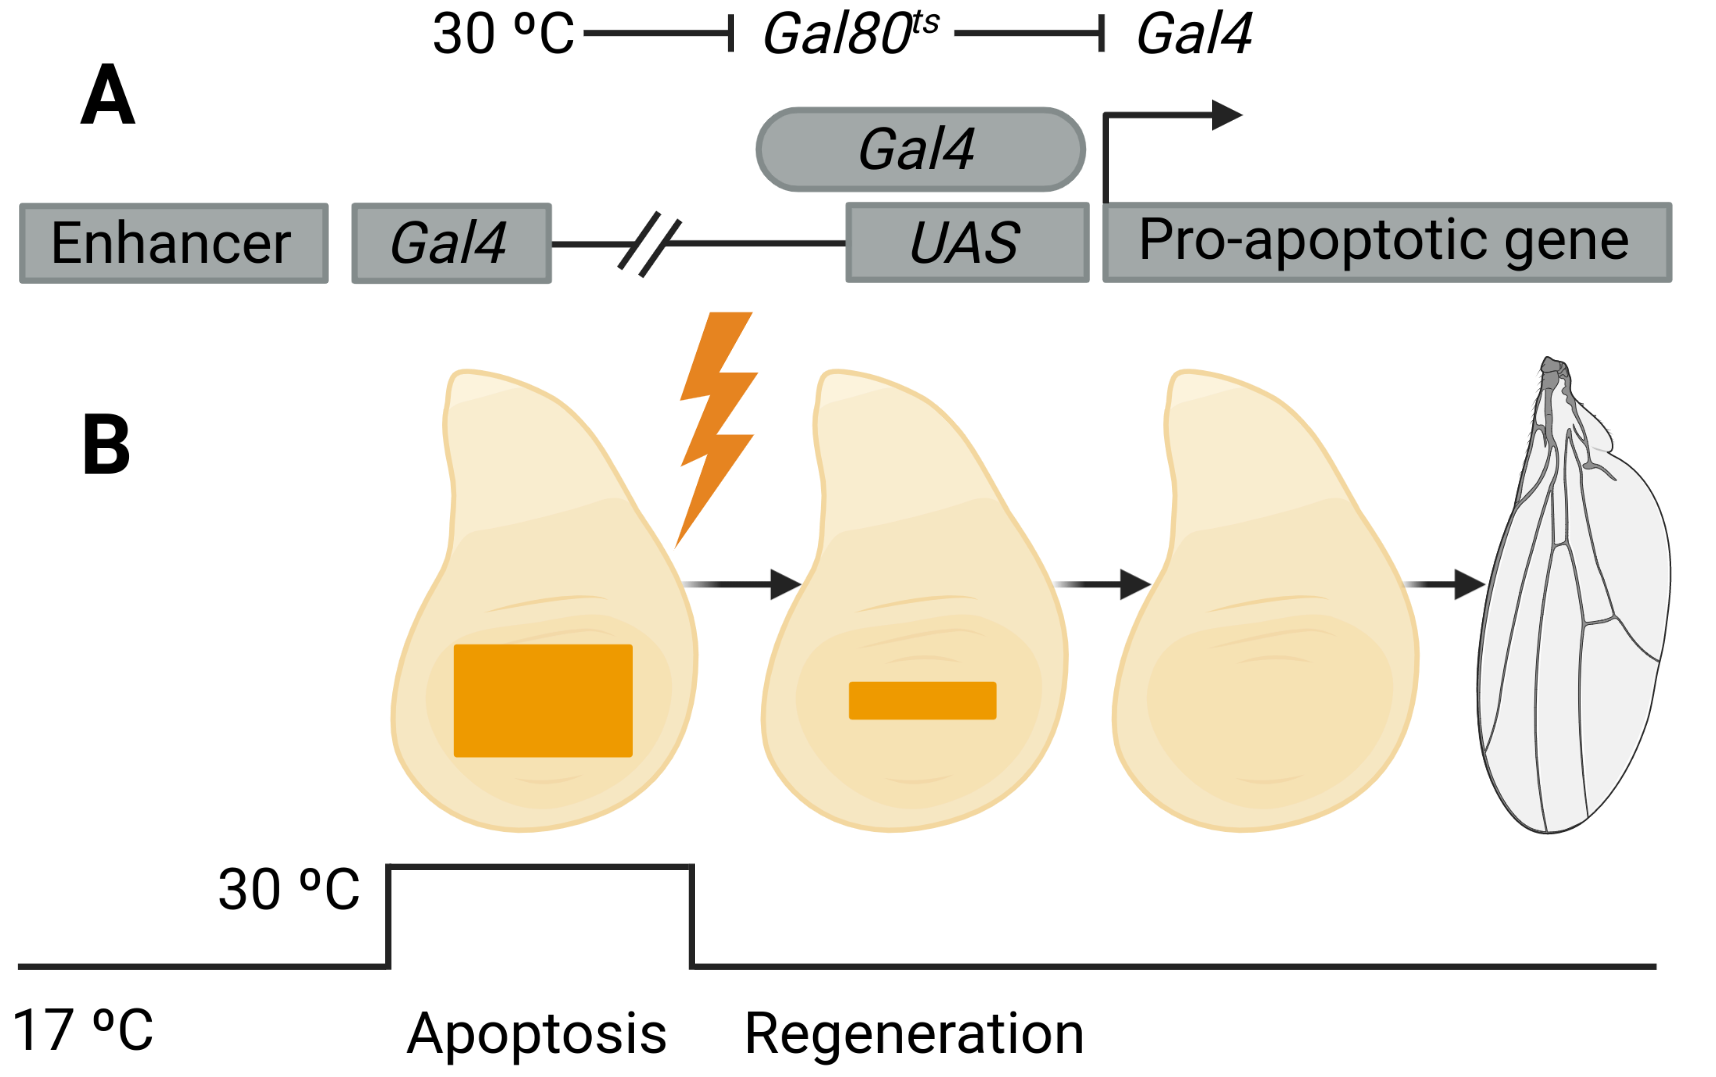
\includegraphics[width=0.55\textwidth]{img/introduction/induction_cell_death.png}
  \caption[Regeneration in \textit{Drosophila} wing imaginal disc]{\textbf{Regeneration in \textit{Drosophila} wing imaginal disc}. \textbf{(A)} Induction of cell-death using the \textit{Gal4/UAS} system, 30ºC inhibits \textit{Gal-80}$^{ts}$ permitting pro-apoptotic gene expression. \textbf{(B)} Regeneration progress of wing imaginal disc, cell-death induction occurs on the wing pouch. Inspired by.\autocite{hariharan_2017_imaginal}}
  \label{fig:imaginal-disc}
\end{figure}

\subsection{LncRNAs involved in regeneration}
\label{sub:lncRNA-reg}

Several recent studies have described roles of chromatin structures, DNA regulatory elements (enhancers and promoters), transcription factors, PCGs, and signaling pathways in regeneration.\autocite{vizcaya_2018,vizcaya_2020_chromatin,santabarbara_2015,blanco_2010} Nonetheless, lncRNAs function and their mechanisms of action in regeneration remain poorly explored, mostly limited to performing transcriptome analyses for PCGs and leaving lncRNAs as an appendix. Some lncRNAs have been unveiled to act in more than one regenerative type. For instance, \textit{H19} and \textit{MALAT1} are involved in skeletal muscle and liver regeneration,\autocite{sergeeva_2020_liver_regeneration,gonccalves_2017_skeletal} whereas \textit{Sirt1AS} is implicated in muscle and cardiac regeneration.\autocite{gonccalves_2017_skeletal,dong_2021_cardiomyocyte}

Following injury, skeletal muscle can regenerate from muscle-specific stem cells, termed satellite cells (SCs), which proliferate and differentiate into myotubes.\autocite{baghdadi_2018_skeletal} \textit{H19} is highly expressed in SCs, and \textit{H19} targeted deletion leads to 50\% loss of SCs in adult mice.\autocite{venkatraman_2013_h19} The mechanism is unknown but it may be linked with the \textit{Igf2}-\textit{Igf1r} signaling pathway.\autocite{gonccalves_2017_skeletal} Moreover, the pro-proliferative \textit{Cdc6} and \textit{Smad} genes are repressed by two miRNAs produced from the first intron of \textit{H19}.\autocite{dey_2014_h19} In liver regeneration, \textit{H19} is upregulated and contributes to the increased expression of the \textit{CcnD1} gene and DNA synthesis, leading to hepatocyte proliferation.\autocite{sergeeva_2020_liver_regeneration}

\textit{MALAT1} is upregulated after 2 hours of liver wound-healing and acts as a regulatory factor in the cell cycle. \textit{MALAT1} participates in the activation of the \textit{Wnt}/$\beta$\textit{-catenin} signaling pathway by inhibiting the \textit{Axin1} and \textit{APC} loci.\autocite{li_2017_malat1} Additionally, \textit{MALAT1} participates in muscle differentiation, acting as a sponge for miR-133; preventing miR-133 from inhibiting its target PCG, such as \textit{SRF}. In consequence, \textit{SRF} is expressed and able to promote terminal differentiation of the muscle progenitor cells.\autocite{han_2015_malat1}

The lncRNA \textit{Sirt1AS} is transcribed from the antisense strand of the PCG \textit{Sirt1}, which is a NAD-dependent class III protein deacetylase. \textit{Sirt1AS} interacts with the 3’UTR of \textit{Sirt1} forming a RNA-RNA duplex to protect \textit{Sirt1} transcript from degradation mediated by miR-34a.\autocite{gonccalves_2017_skeletal,dong_2021_cardiomyocyte} Thus, \textit{Sirt1} stability and pro-proliferation ability are augmented. During muscle regeneration, \textit{Sirt1AS} transcription sustains muscle-progenitor-cell proliferation by increasing the expression of cyclins B, D, and E.\autocite{wang_2016_sirt1,wang_2014_sirt1} Moreover, loss-or-function results in mice suggest \textit{Sirt1AS} is required and sufficient to induce cardiomyocyte proliferation (mechanism needed for heart regeneration). Additional results in cardiac regeneration demonstrated that \textit{Sirt1AS} overexpression enhances survival rate, improves cardiac function, and inhibits fibrosis after myocardial infarction.\autocite{dong_2021_cardiomyocyte}

Additional lncRNAs have been uncovered to function in different regeneration types including muscle, cardiac, liver, and nerve regeneration in diverse model organisms (see \autoref{tab:lncRNA-example.reg}). Acting in a wide-range of mechanisms, for instance acting as a source of miRNAs (\textit{H19}), acting as a sponge of miRNAs (\textit{MALAT1}, \textit{NR-045363}, \textit{LUCAT1}, \textit{CAREL}), encoding functional peptides from smORFs (\textit{LINC00961}), promoting chromatin loops ($^{ce}$\textit{eRNA}), forming RNA-RNA duplexes (\textit{Sirt1AS}), inhibiting or activating the expression \textit{in cis} or \textit{in trans} of neighboring PCGs (\textit{Dum}, \textit{SRA}, \textit{CPR}, \textit{lncPHx2}, \textit{lncHand2}, \textit{Silc1}),  and activating signaling pathways (\textit{ECRAR}, \textit{lncDACH1}, \textit{LALR1}). See \autocite{gonccalves_2017_skeletal,dong_2021_cardiomyocyte,goldman_2020_tissue_regeneration,baghdadi_2018_skeletal,sergeeva_2020_liver_regeneration} for further details.

\begin{table}[!htb]
  \caption[Mechanisms of action of lncRNAs involved in tissue regeneration]{\textbf{Mechanisms of action of lncRNAs involved in regeneration}}
  \begin{scriptsize}
    \begin{tabulary}{0.65\linewidth}{lll}
      \textbf{LncRNA} & \textbf{Regeneration type} & \textbf{Mechanism} \\ \hline
      \textit{H19}\autocite{dey_2014_h19} & Skeletal muscle and liver regeneration & Acts as a source of miRNAs\\
      \textit{MALAT1}\autocite{li_2017_malat1} & Skeletal muscle and liver regeneration & Acts as a sponge for miR-133\\
      \textit{Sirt1AS}\autocite{dong_2021_cardiomyocyte} & Skeletal muscle and cardiac regeneration & Inhibits \textit{Sirt1} degradation \\
      \textit{Dum}\autocite{gonccalves_2017_skeletal} & Skeletal muscle regeneration & Inhibits \textit{Dppa2} expression \\
      $^{ce}$\textit{eRNA}\autocite{gonccalves_2017_skeletal} & Skeletal muscle regeneration & Increases \textit{MyoD} expression \\
      \textit{SRA}\autocite{gonccalves_2017_skeletal} & Skeletal muscle regeneration & Co-activator of \textit{MyoD}\\
      \textit{LINC00961}\autocite{gonccalves_2017_skeletal} & Skeletal muscle regeneration & Contains a smORF that encodes for \textit{SPAR}\\
      \textit{ECRAR}\autocite{dong_2021_cardiomyocyte} & Cardiac regeneration & Promotes cardiomyocytes to re-enter cell-cycle \\
      \textit{NR-045363}\autocite{dong_2021_cardiomyocyte} & Cardiac regeneration & Acts as a sponge for miR-216\\
      \textit{LUCAT1}\autocite{dong_2021_cardiomyocyte} & Cardiac regeneration & Acts as a sponge for miR-612\\
      \textit{lncDACH1}\autocite{dong_2021_cardiomyocyte} & Cardiac regeneration & Bounds to \textit{PP1A} subunit\\
      \textit{CPR}\autocite{dong_2021_cardiomyocyte} & Cardiac regeneration & Inhibits \textit{MCM3} expression\\
      \textit{CAREL}\autocite{cai_2018_carel} & Cardiac regeneration & Acts as a sponge for miR-296\\
      \textit{LALR1}\autocite{sergeeva_2020_liver_regeneration} & Liver regeneration & Activates the \textit{Wnt}/$\beta$\textit{-catenin} pathway\\
      \textit{lncPHx2}\autocite{sergeeva_2020_liver_regeneration} & Liver regeneration & Activates \textit{E2F1} and histone proteins expression\\
      \textit{lncHand2}\autocite{sergeeva_2020_liver_regeneration} & Liver regeneration & Upregulates \textit{c-Met} expression \\
      \textit{Silc1}\autocite{goldman_2020_tissue_regeneration} & Nerve regeneration & Upregulates \textit{Sox11} expression\\
    \end{tabulary}
  \end{scriptsize}
  \label{tab:lncRNA-example.reg}
\end{table}

To the best of our knowledge, most of the work performed about tissue regeneration in \textit{Drosophila} imaginal discs has been focused mainly on the chromatin, transcription factor, signaling pathways, and PCGs level.\autocite{vizcaya_2018,vizcaya_2020_chromatin,santabarbara_2015,blanco_2010} And little work has been performed in the literature to characterize the role and mechanisms of action of lncRNAs in fruit fly discs during regeneration. 

\clearpage


